\documentclass[paper=a4paper,jafontsize=9pt,head_space=15mm,gutter=20mm,
twocolumn,number_of_lines=49, line_length=26zw]{myuarticle}

\begin{document}

\title{{\LARGE\bfseries\gtfamily 環境情報のセンシングを用いた他者の環境評価を表現するロボットシステム}}
\author{\\\ 22120165 中村龍造 \\ (指導教員 : 佐藤宏樹)\\ \\}
\date{}
\maketitle

\section{はじめに}
私たちの周りには、人間以外にも多くの存在が共存している。それらの存在は、それぞれ独自の感覚や基準で環境を捉えているが、私たちはその感覚を直接共有することができない。このような「他者」の経験を理解し、共感することは、多様な存在との共生を考える上で重要な課題となっている。

本稿では、取得した環境データに対して、人間、動植物、非生物などといった複数の他者からの評価基準を設定し、評価結果をロボットの身体的動作を通して表現するシステム(以下「本システム」)を提案する。本システムを通じて、ユーザーが他者にとっての快適さを知り、他者への理解、関心を深めることで、多様な存在との対話の機会創出を目指す。

\section{関連研究と課題}

環境センシング分野では,IoTやセンサー技術の発展により,室内環境の継続的なモニタリングが可能となっており\cite{Saini-2020-IndoorAirQualityMonitoring},個々人の主観による評価も必要とされている\cite{Coulby-2020-ScopingReviewTechnologicalApproaches}.

他者視点の表現に関する取り組みとしては,「In the Eyes of the
Animal」\cite{Dezeen-2015-MarshmallowLaserFeastsEyes}やrapoptosis\cite{--ソンヨン}がある.また,Human
Robot
Interactionの分野では,Breazeal\cite{C.Breazeal-2004-SocialInteractionsHRIRobot}が人間と協働するパートナーとしてのロボットのあり方を提示している.

以上から本研究では,人間,動植物,非生物など,様々な他者を基準に,それらから見た環境の快・不快を,ロボットの身体的動作で表現するシステムを開発する.

\section{システム要件}
本システムの開発にあたって,次の3点を要件とする.
\begin{itemize}
  \item ロボット:自身が代弁する他者の特徴が動きに現れている
  \item 評価システム:他者基準の評価が適切に行われる
  \item 全体:ユーザー自身とそれ以外との環境の受け取り方の違いを体験することができる
\end{itemize}

\subsection{全体のフロー}
本システムは,ユーザー,環境,センサー,ロボット,本システムの5つからなる.システム全体のフローを図\ref{fig:system-flow}に示す.

\fboxsep=0pt            %画像と枠線をくっつける.
\fboxrule=1pt            %枠線の太さを1ptにする.
\begin{figure}[h]
  \centering
  \fbox{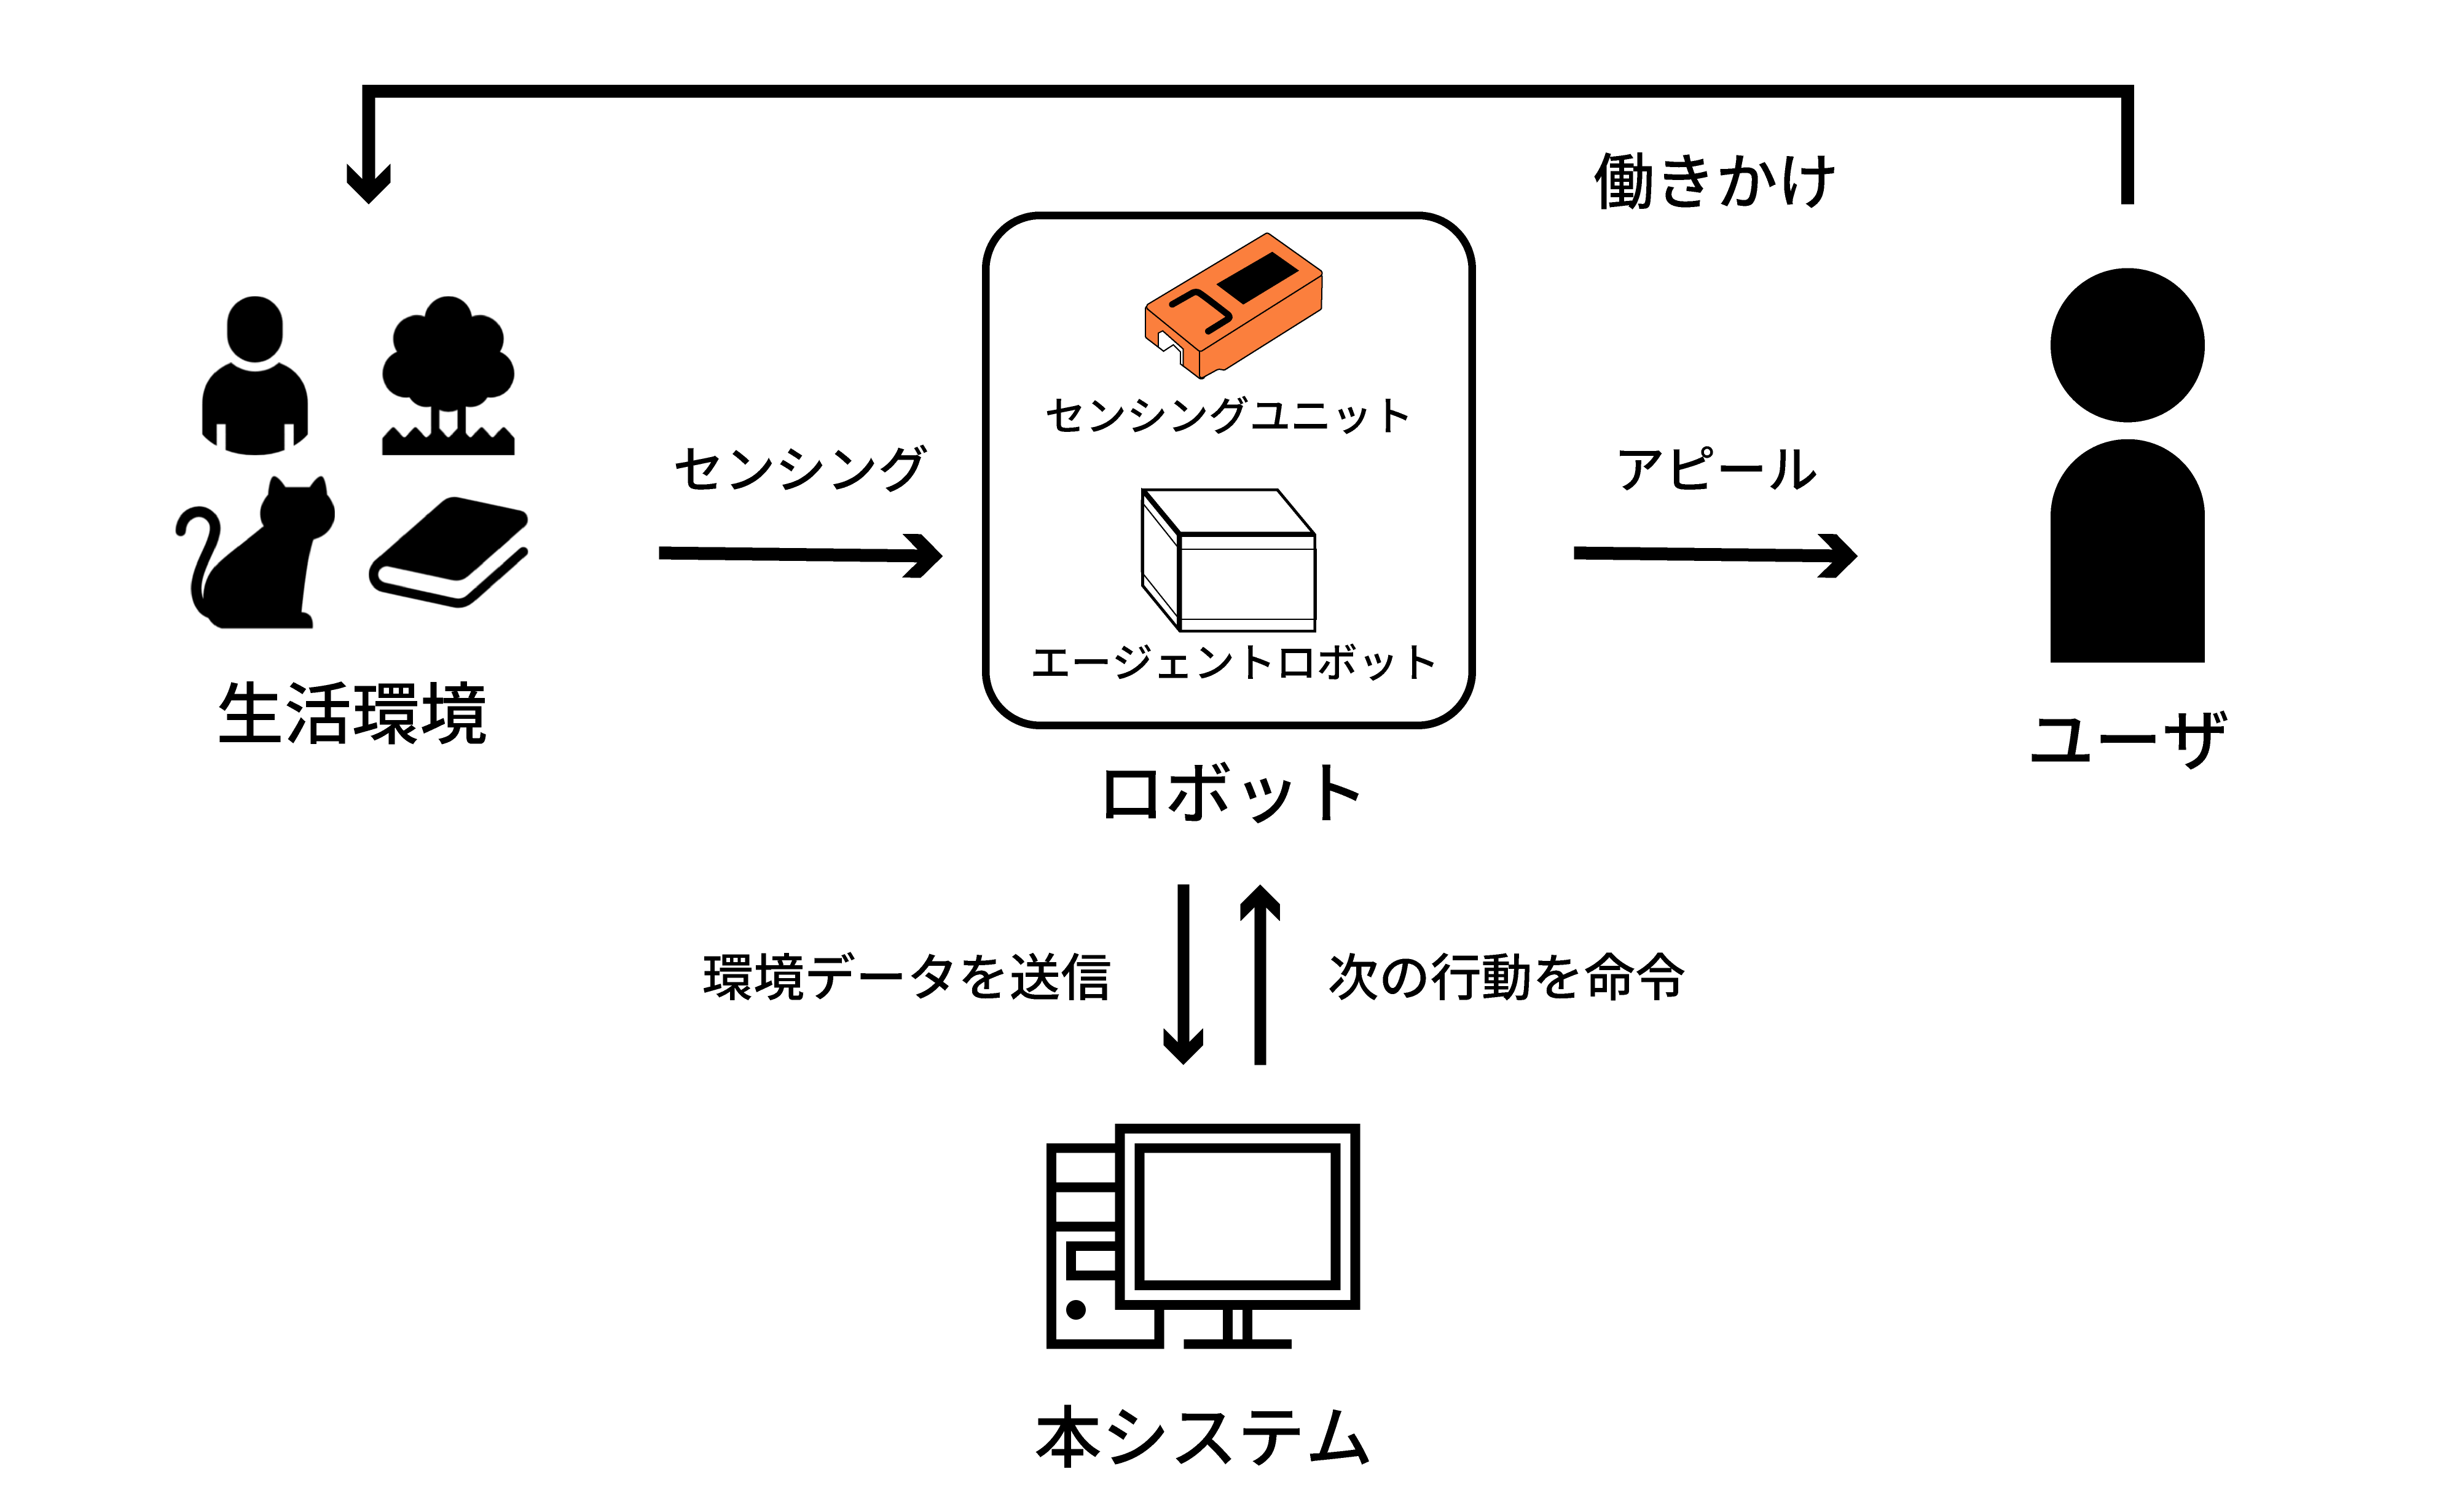
\includegraphics[keepaspectratio, clip,
  width=0.8\columnwidth]{resources/system_flow.png}}
  \caption{システム全体のフロー図}
  \label{fig:system-flow}
\end{figure}

はじめに本システムが,センサーを通じて生活空間の環境データを取得する.他者を基準とした評価,評価に応じて快・不快をアピールするなどの行動命令を現実空間のロボットに送信する.ロボットは行動命令に従って人間にアピールする.それを見た人間が環境や他者に対して働きかけることで,他者にとってより快適な環境を得る.

\section{本システムの実装}
本システムは,センシングシステム,評価システム,アクション生成システム,ロボット制御システムから構成される.ハードウェアは,センシングデバイスにM5StickC(M5Stack社)を,ロボットにtoio(SONY社)を用いた.

本システムによってロボットが動作している様子を図\ref{tab:theme-test}に示す.今回の動作検証では,人間の気温,猫の気温,バナナの気温および湿度の3テーマを設定した.人間の適温は18~28℃\cite{JianZhuWuHuanJingWeiShengGuanLiJiZhunnituite|HouShengLaoDongSheng},猫の適温は30~38℃\cite{stellaEnvironmentalAspectsDomestic2016}と設定した.バナナは生育状態ではなく,室内で食品として保存する場合として,気温を14~20℃\cite{--バナナの},湿度を45~85\%\cite{--JISZ87031983試験}とした.

% 実験風景
\setcounter{figure}{2}
\begin{figure*}[t]
  \centering
  \label{tab:theme-test}
  \begin{tabular}{|c|c|c|c|c|}
    \hline
    % 1行目
    \sffamily ペットと遊ぶ                                                & \sffamily 充電ドックに戻る & \sffamily ちょっかいをかける & \sffamily ゴミを発見する & \sffamily その他 \\
    \hline \hline
    % 2行目
    \begin{minipage}[c]{0.15\textwidth}
      \centering
      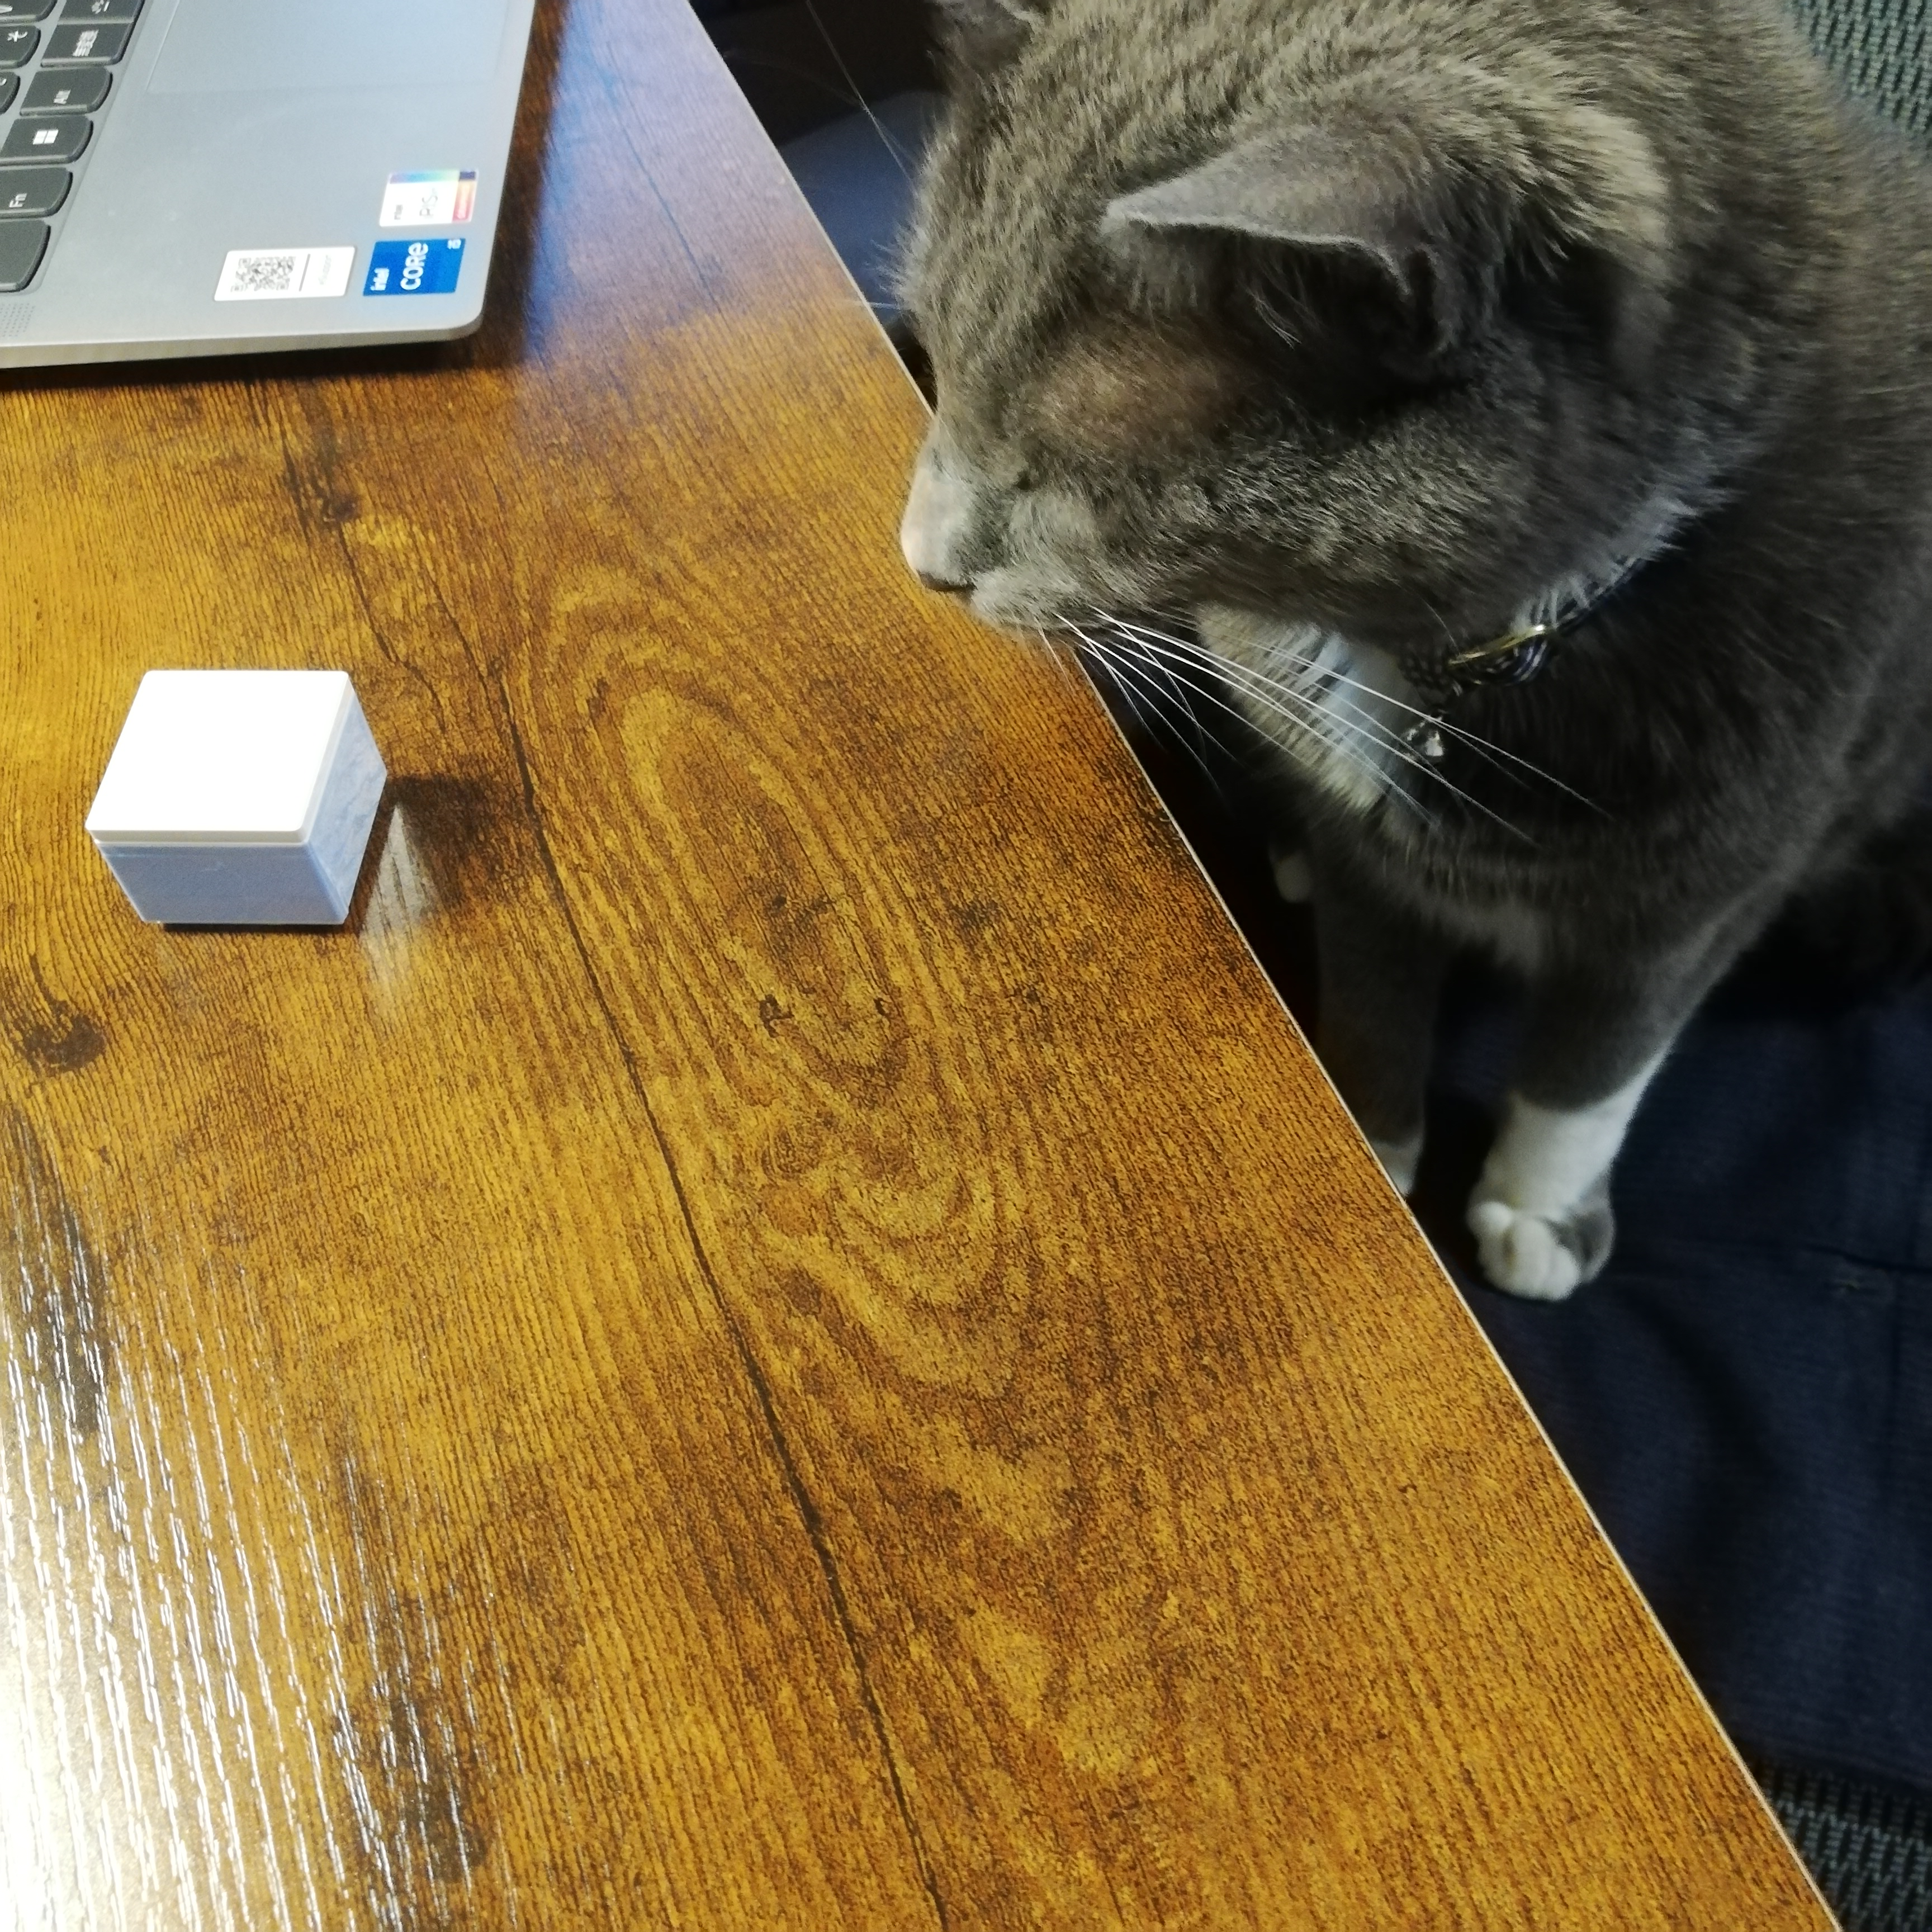
\includegraphics[width=0.9\textwidth]{resources/cat_before.jpg}
    \end{minipage}    &
    \begin{minipage}[c]{0.15\textwidth}
      \centering
      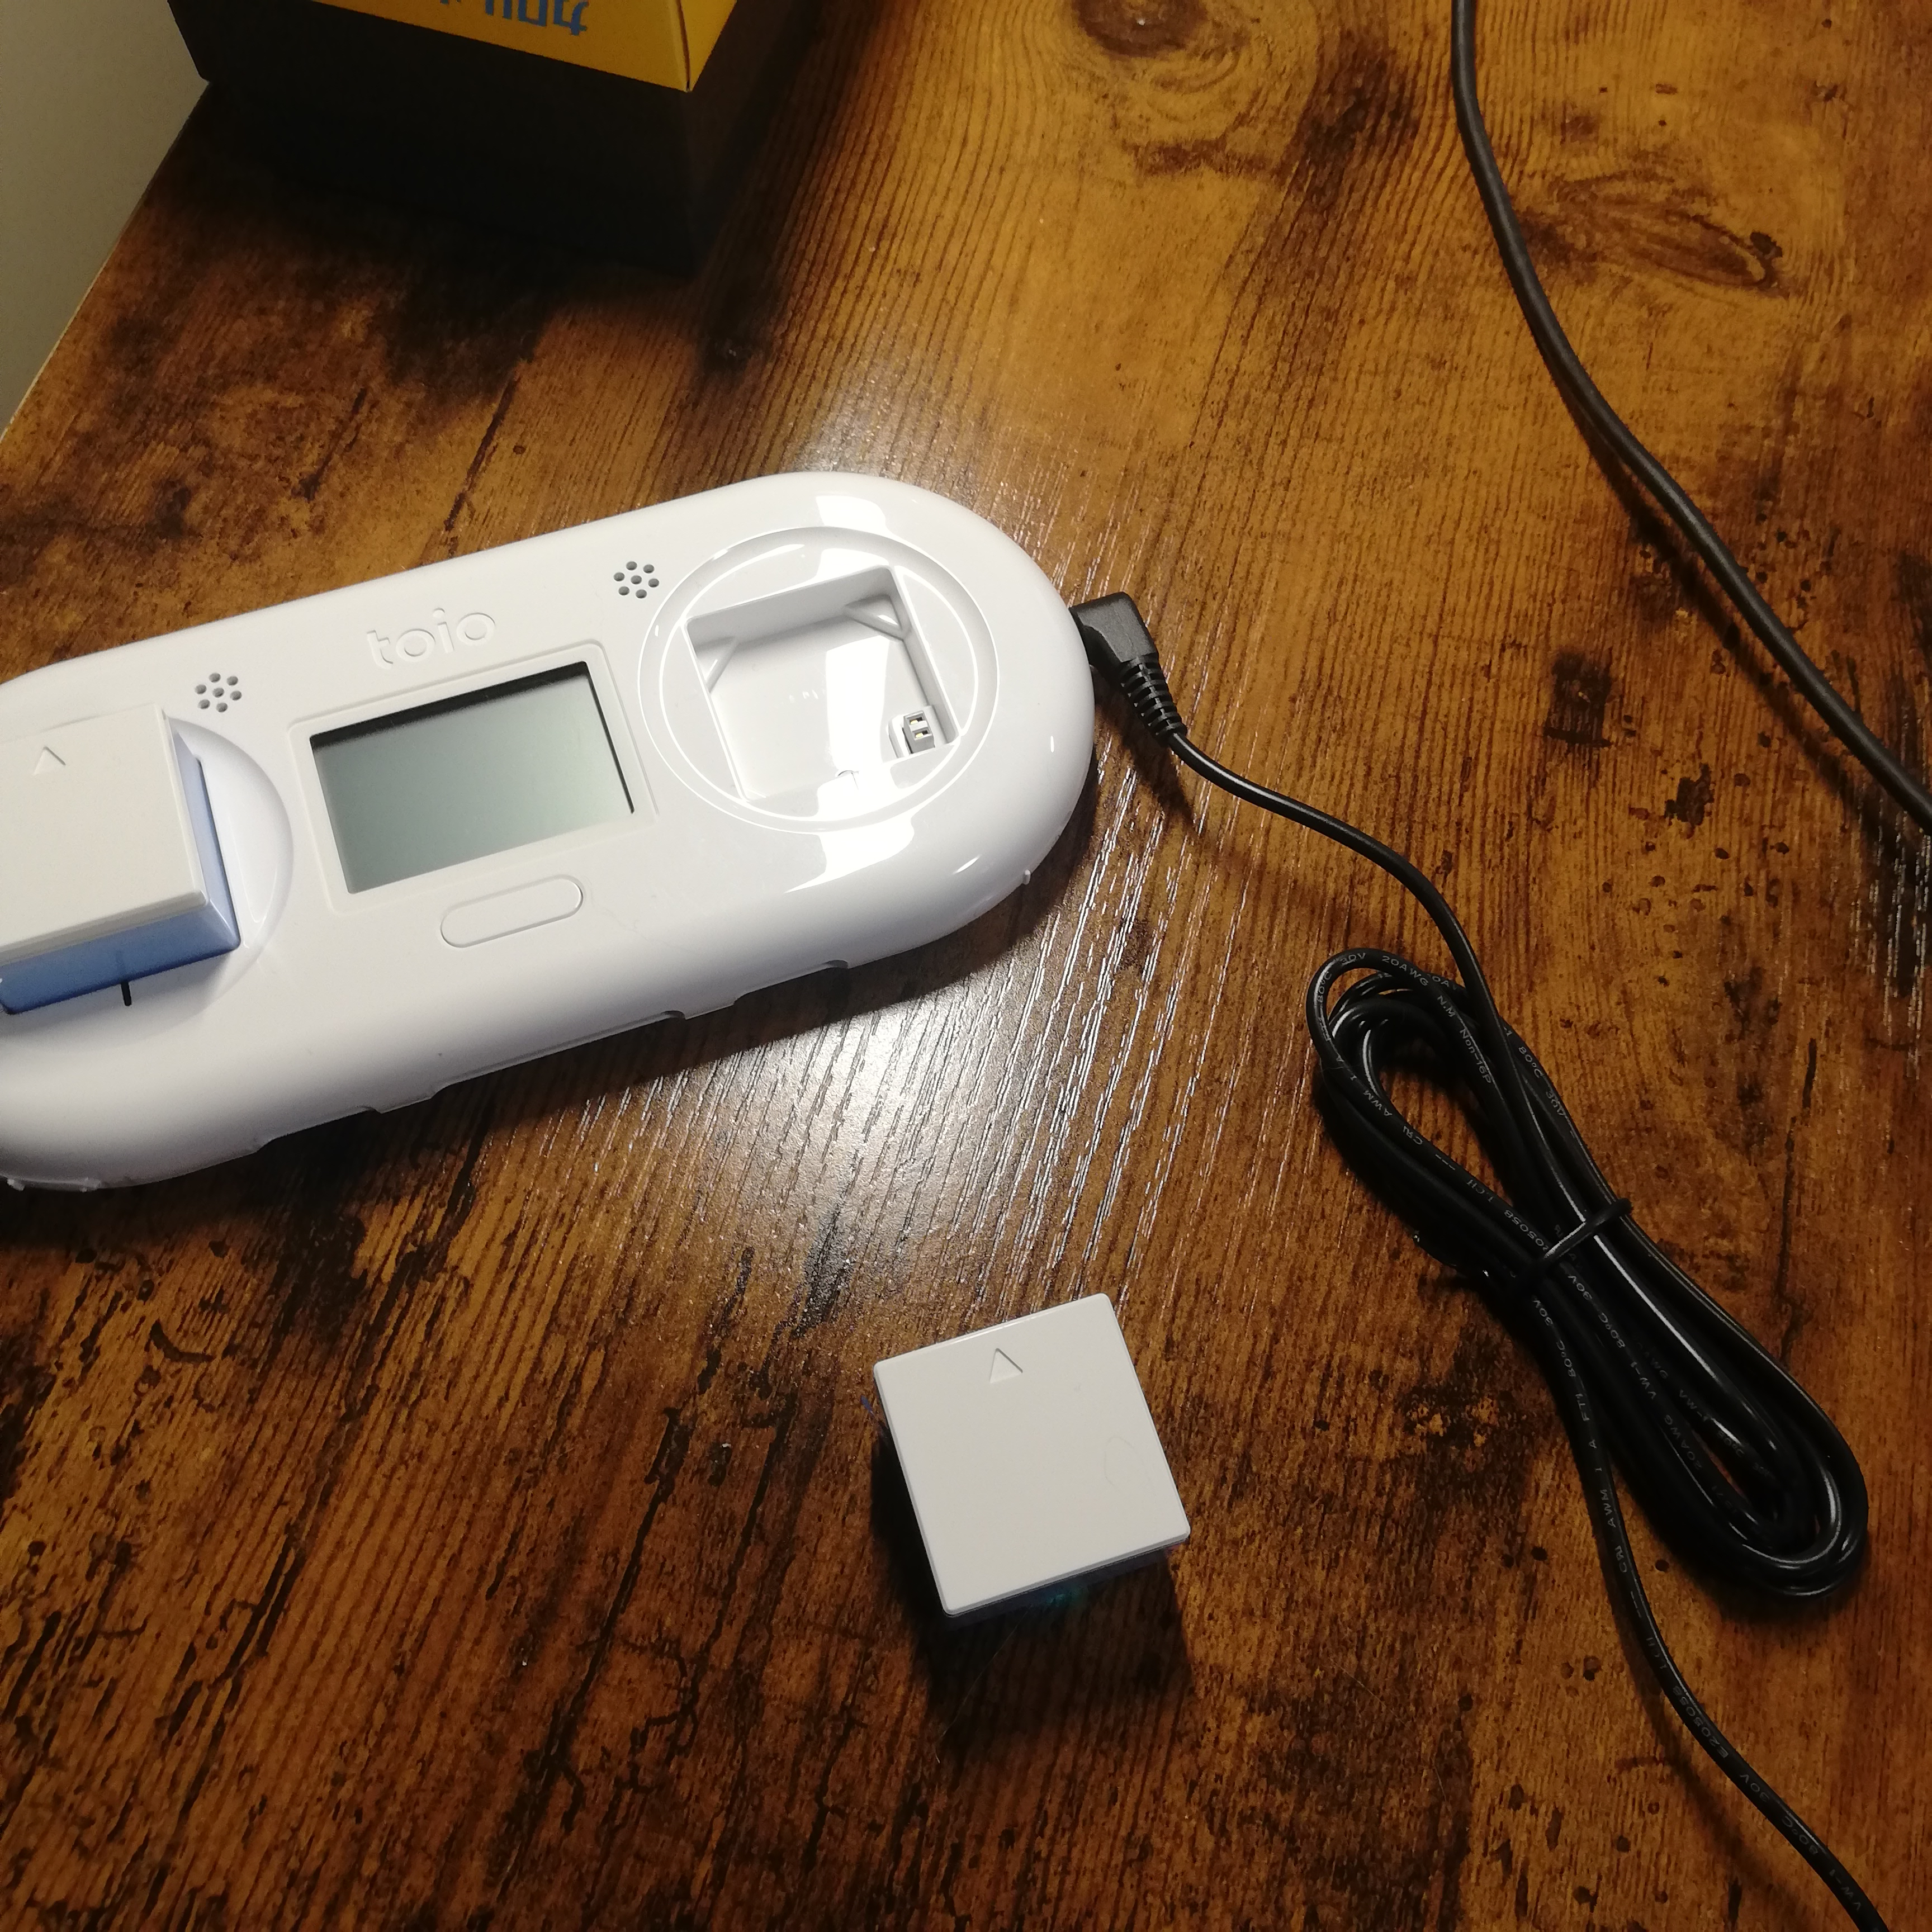
\includegraphics[width=0.9\textwidth]{resources/doc_before.jpg}
    \end{minipage}    &
    \begin{minipage}[c]{0.15\textwidth}
      \centering
      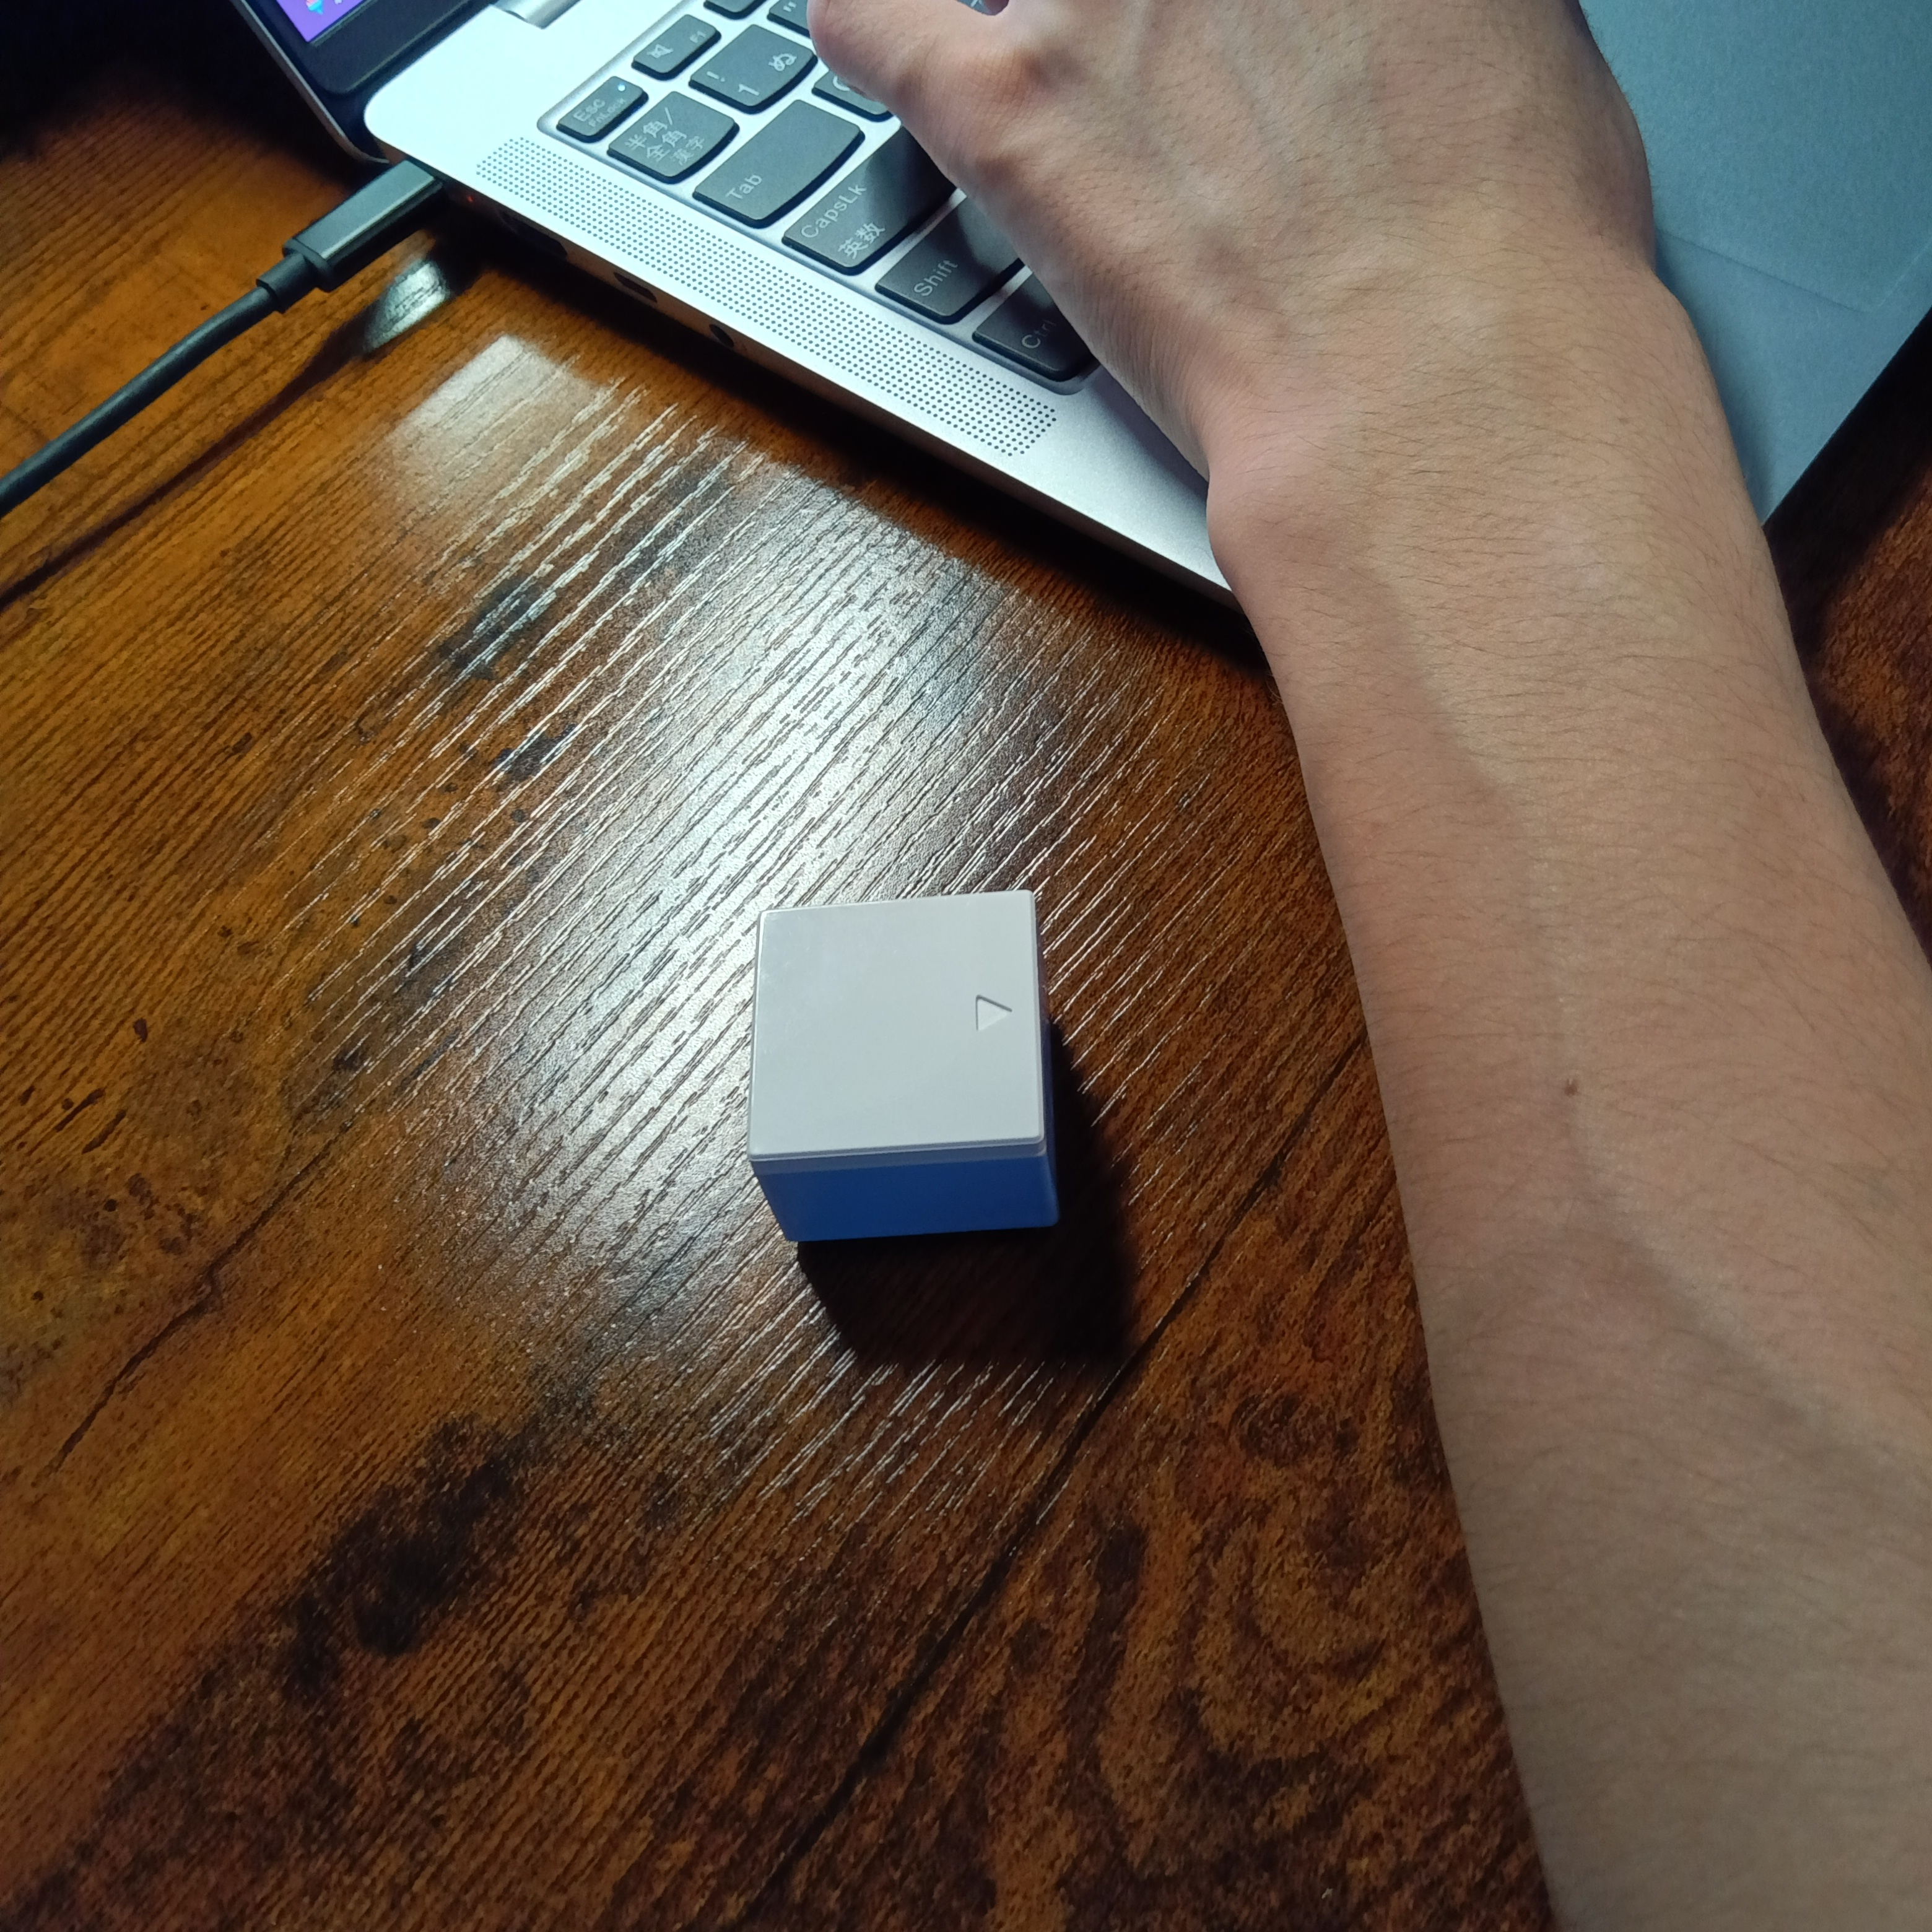
\includegraphics[width=0.9\textwidth]{resources/pet_before.jpg}
    \end{minipage}    &
    \begin{minipage}[c]{0.15\textwidth}
      \centering
      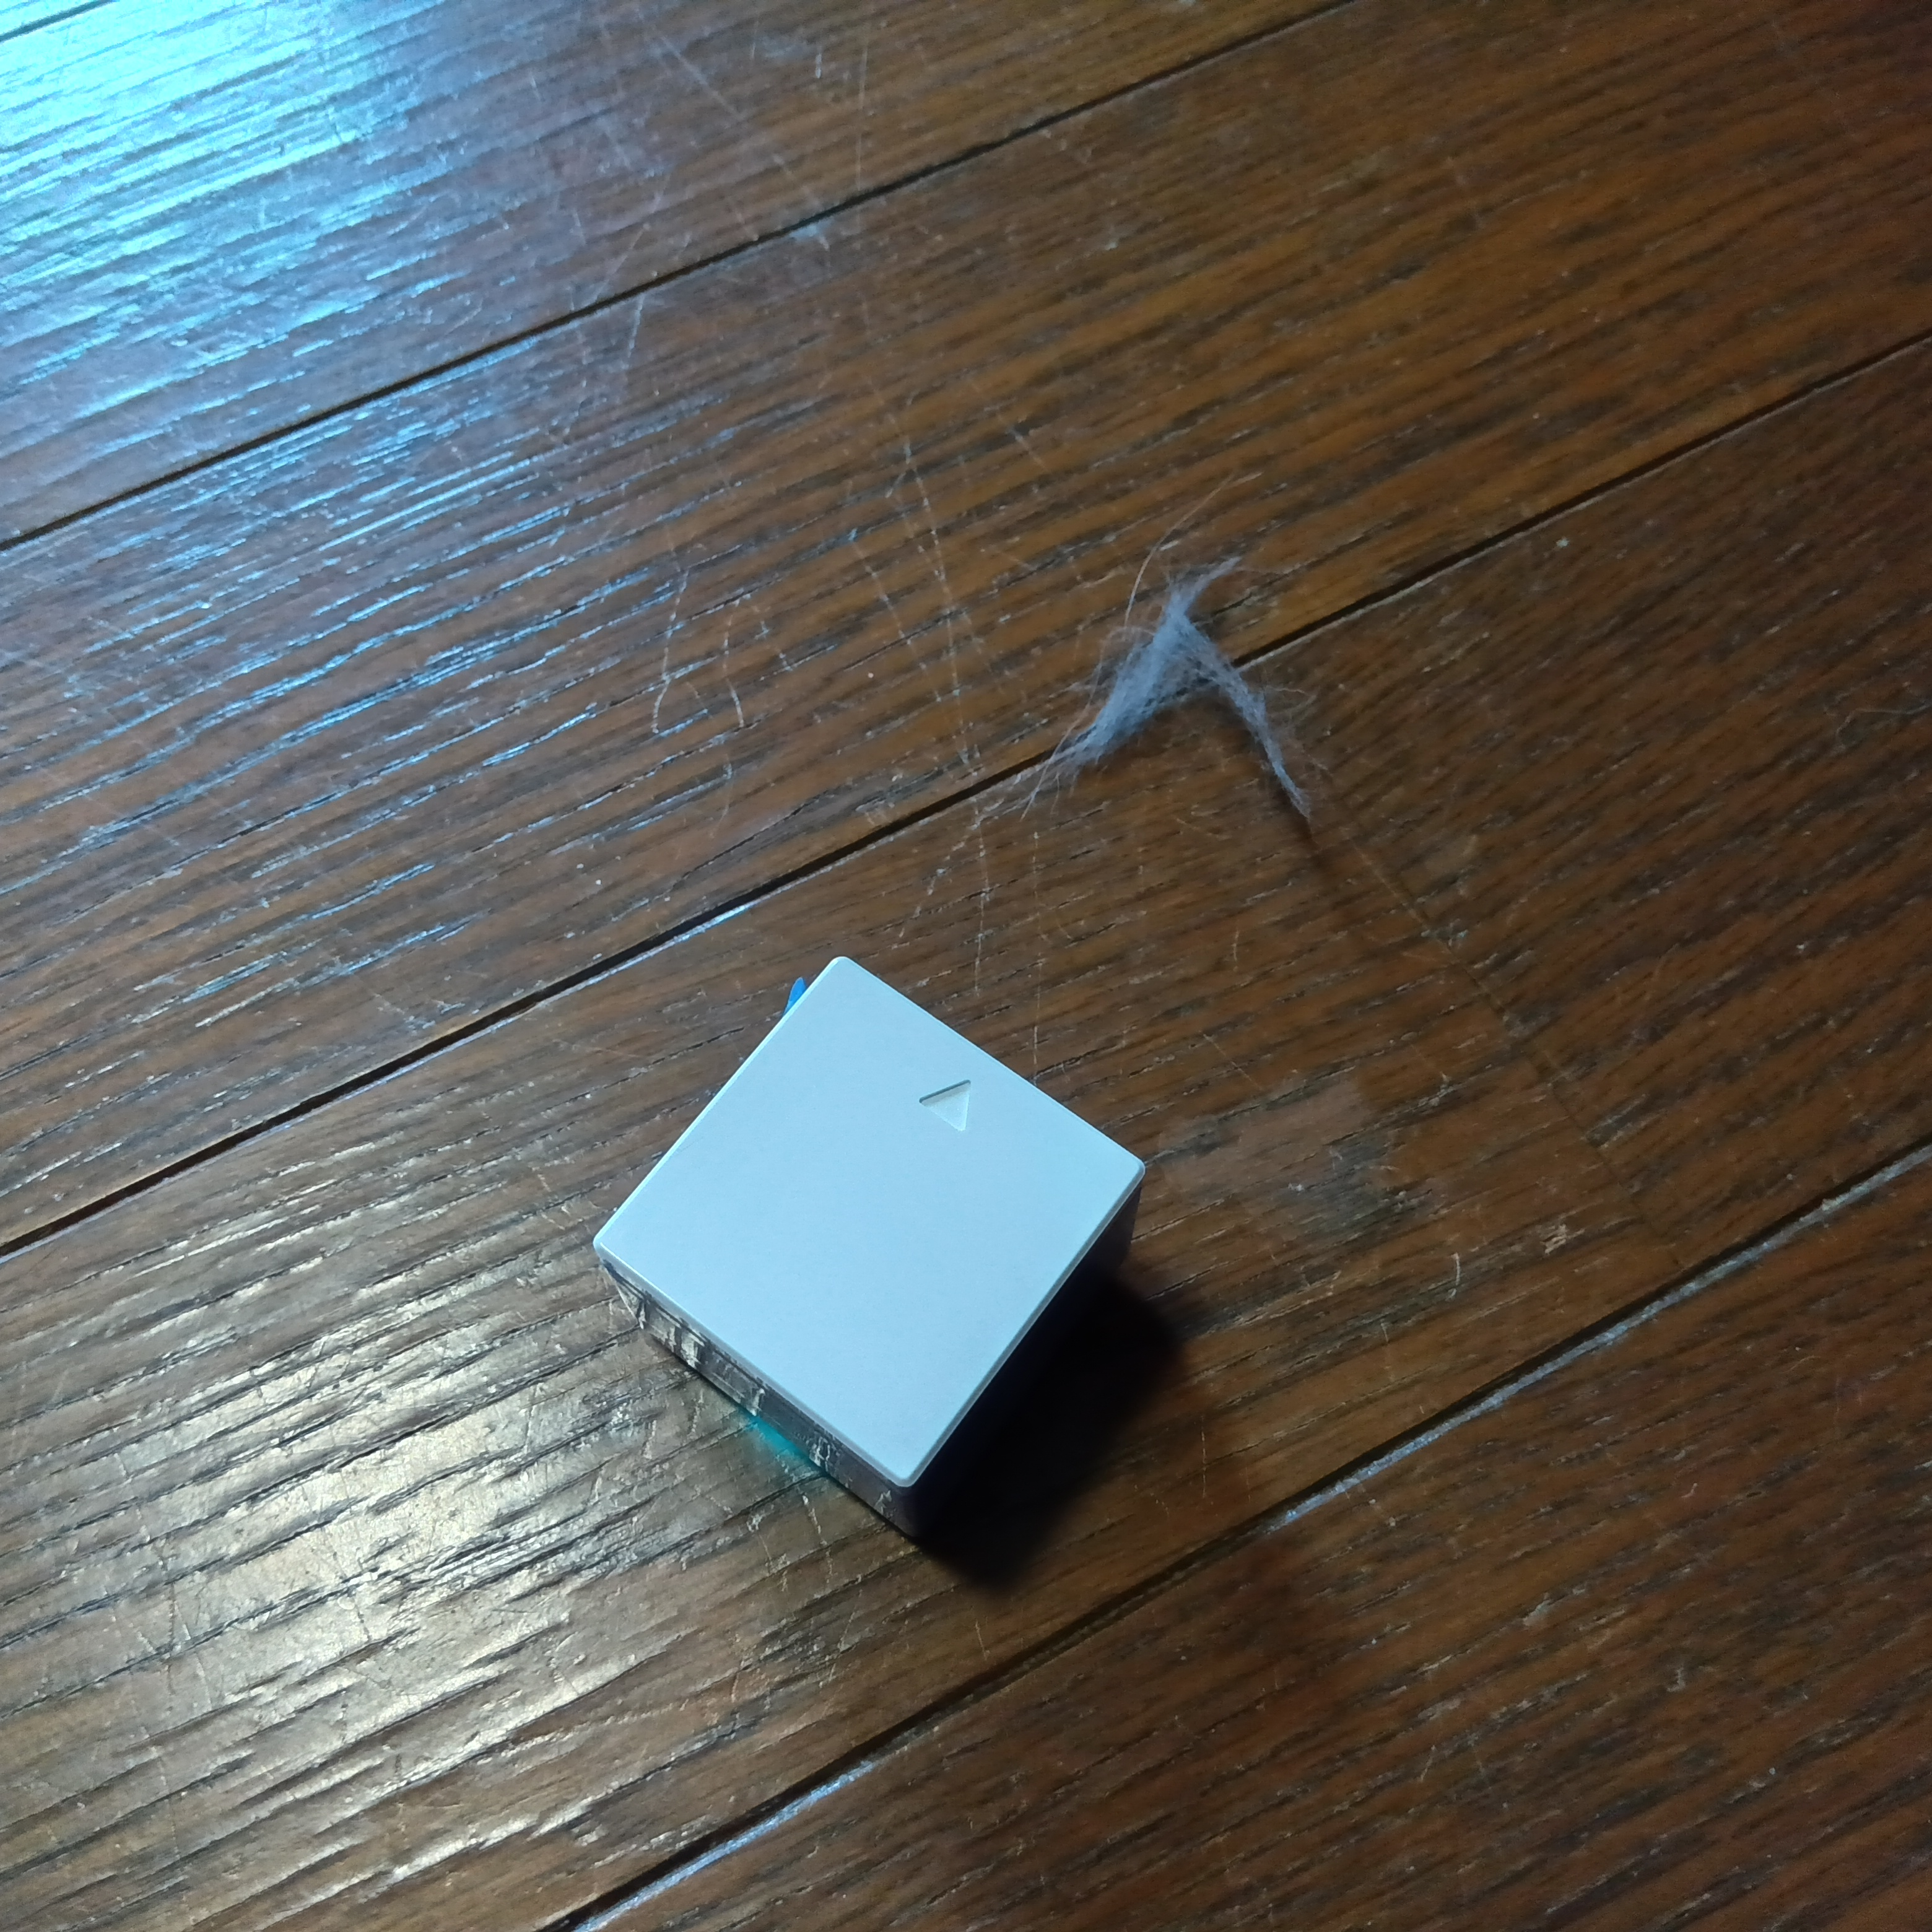
\includegraphics[width=0.9\textwidth]{resources/vacuum_before.jpg}
    \end{minipage} &
    \begin{minipage}[c]{0.15\textwidth}
      \centering
      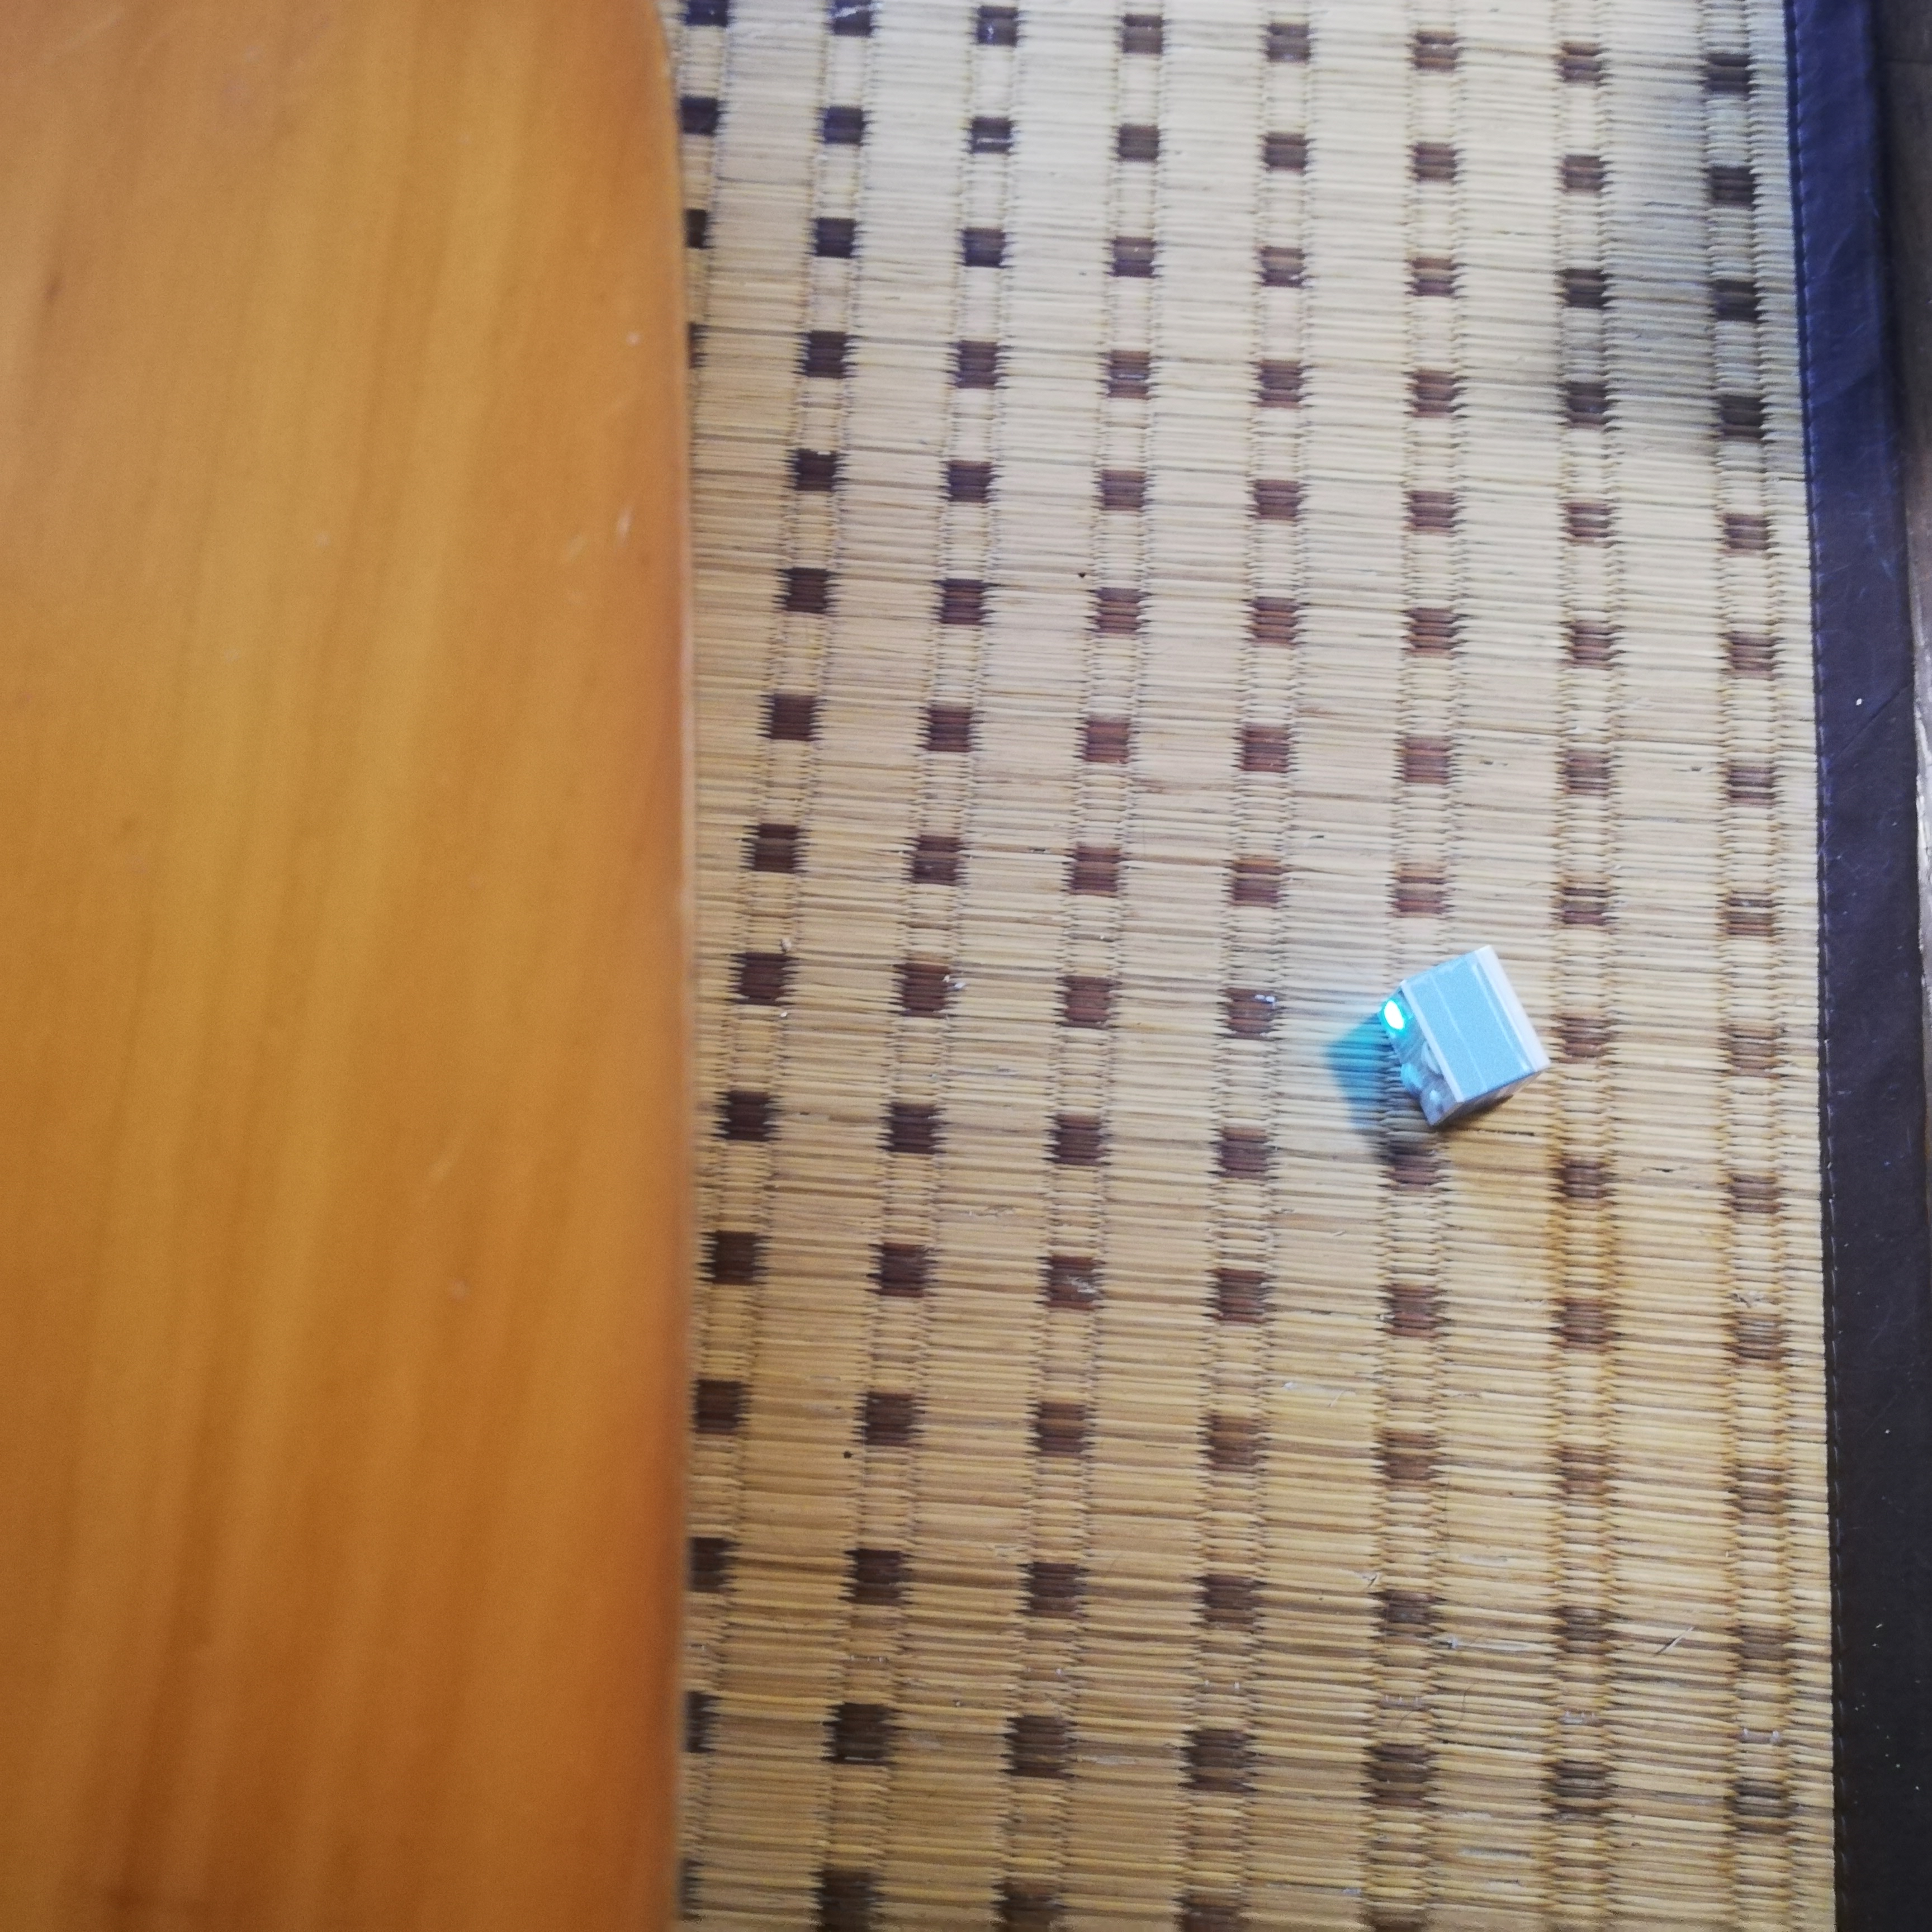
\includegraphics[width=0.9\textwidth]{resources/fall.jpg}
    \end{minipage}
    \\ \hline
    % 3行目
    \begin{minipage}[c]{0.15\textwidth}
      \centering
      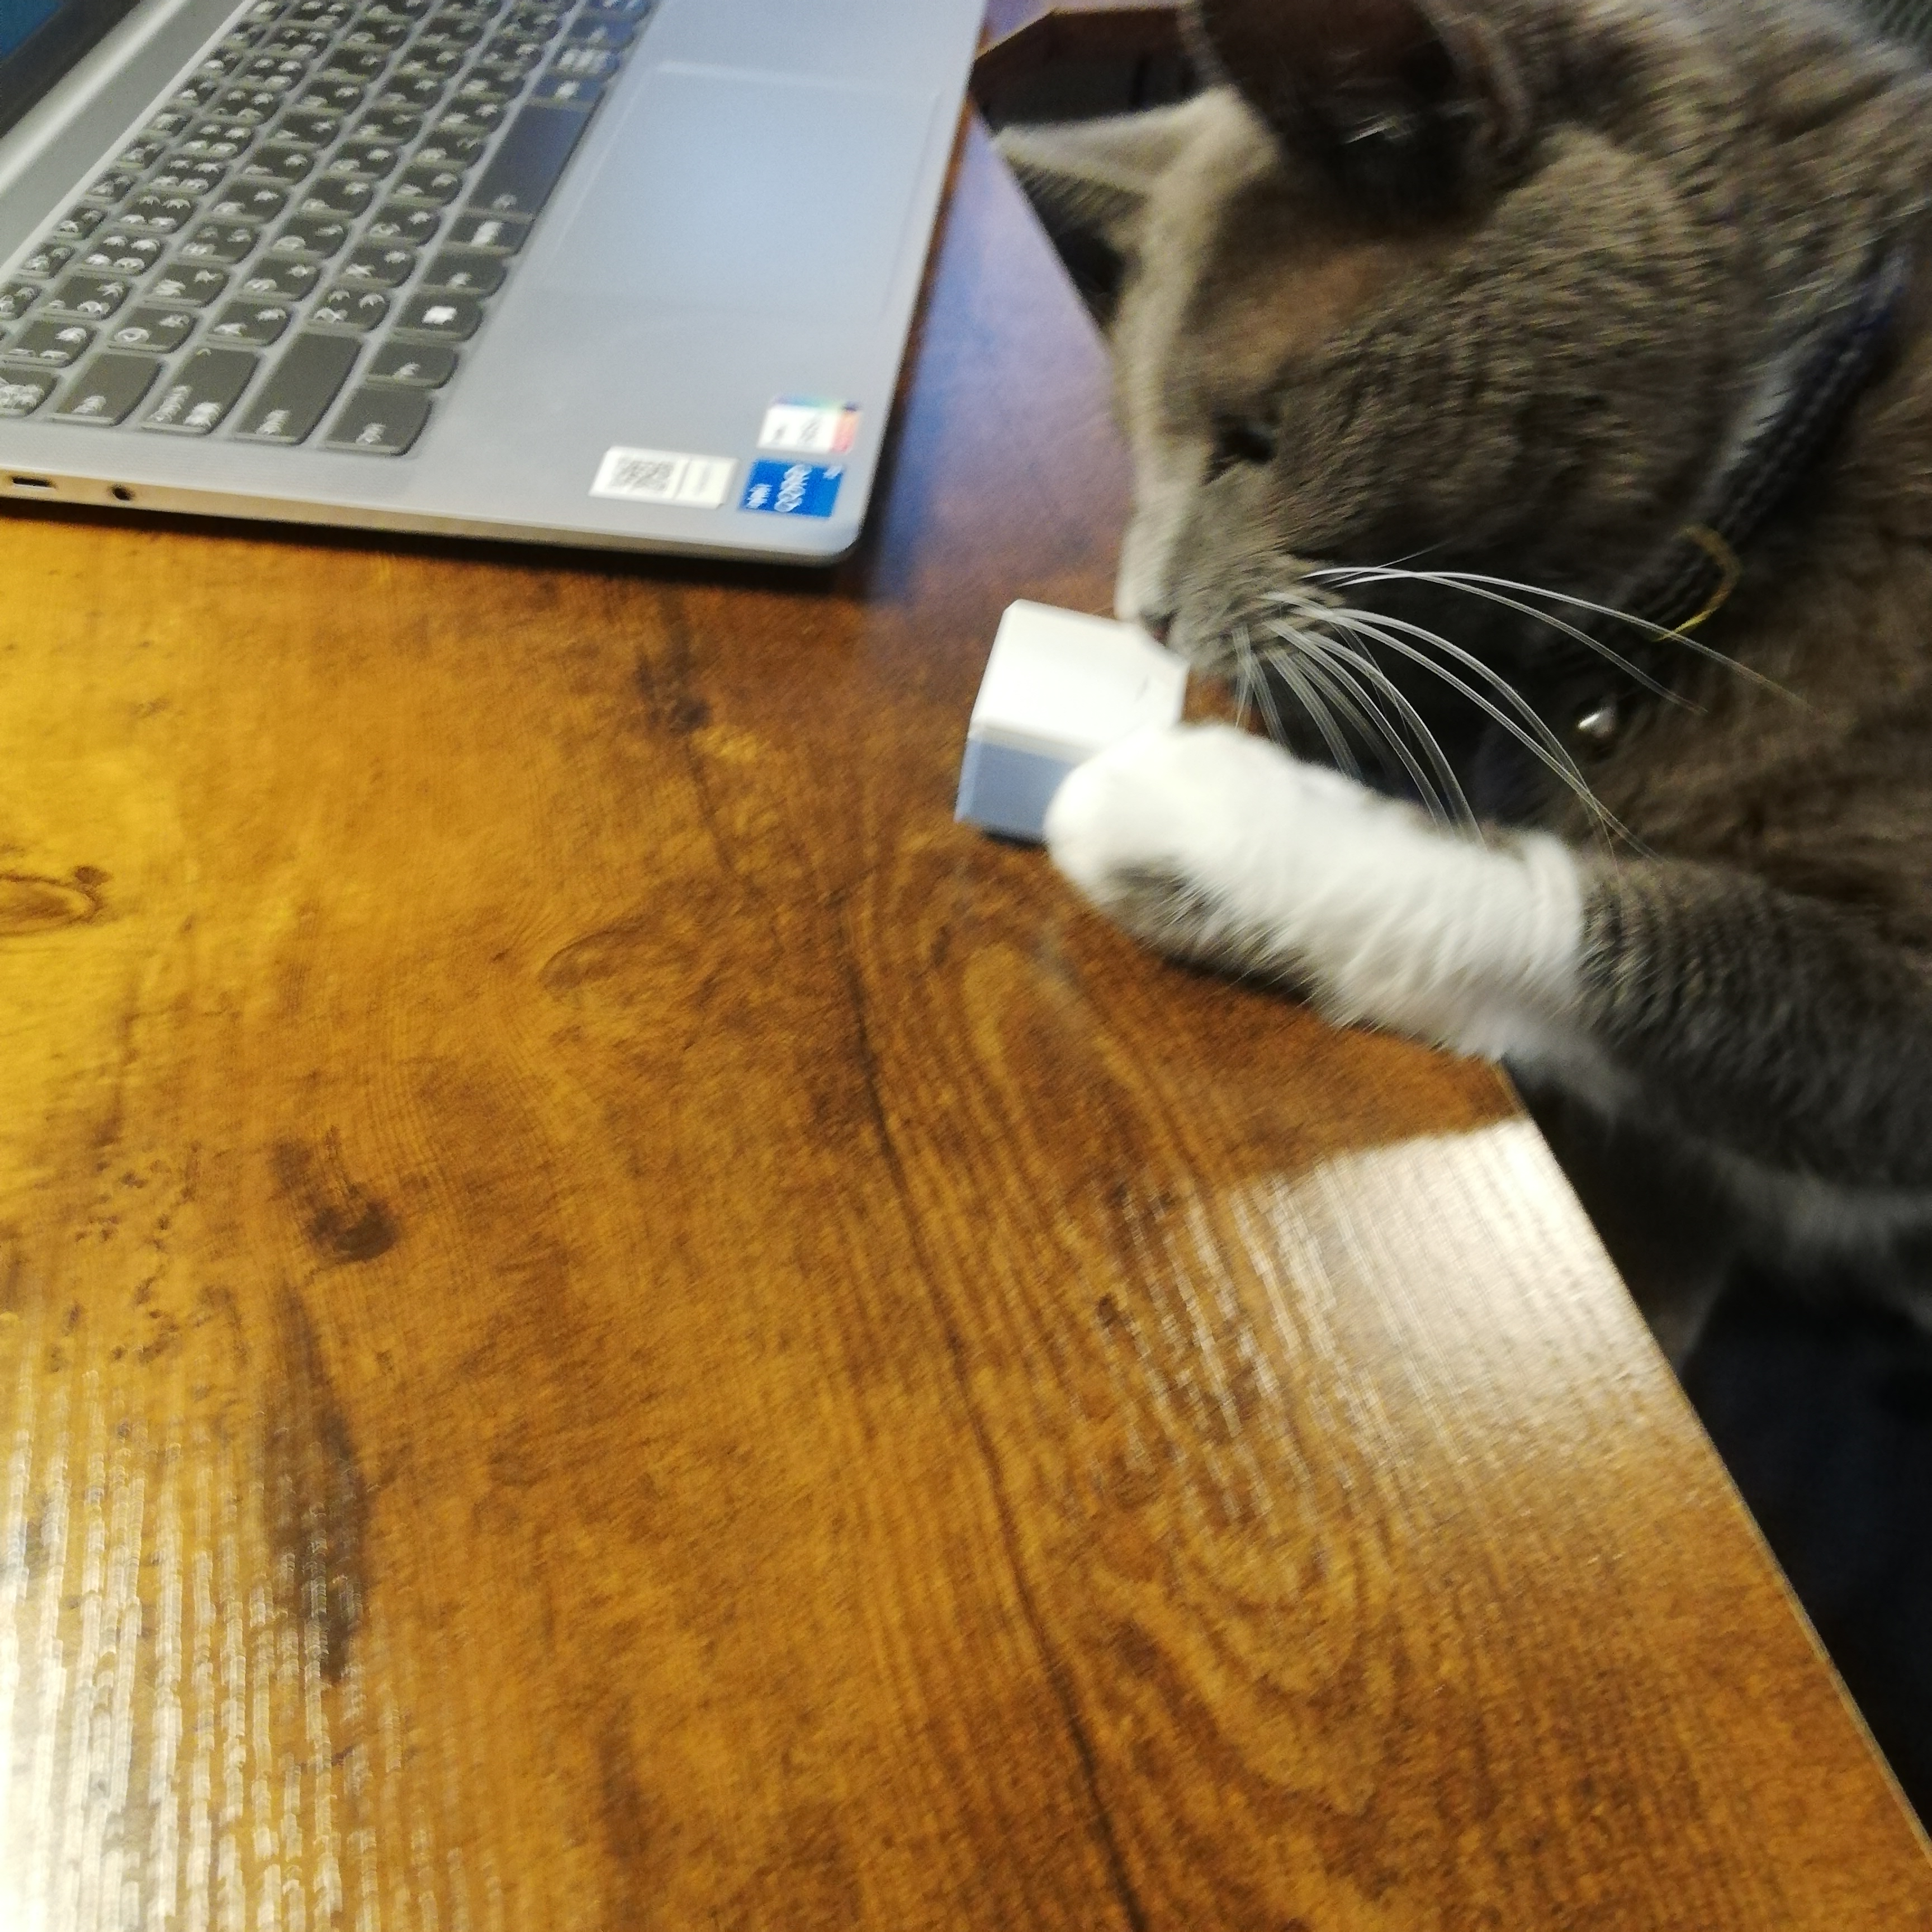
\includegraphics[width=0.9\textwidth]{resources/cat_after.jpg}
    \end{minipage}     &
    \begin{minipage}[c]{0.15\textwidth}
      \centering
      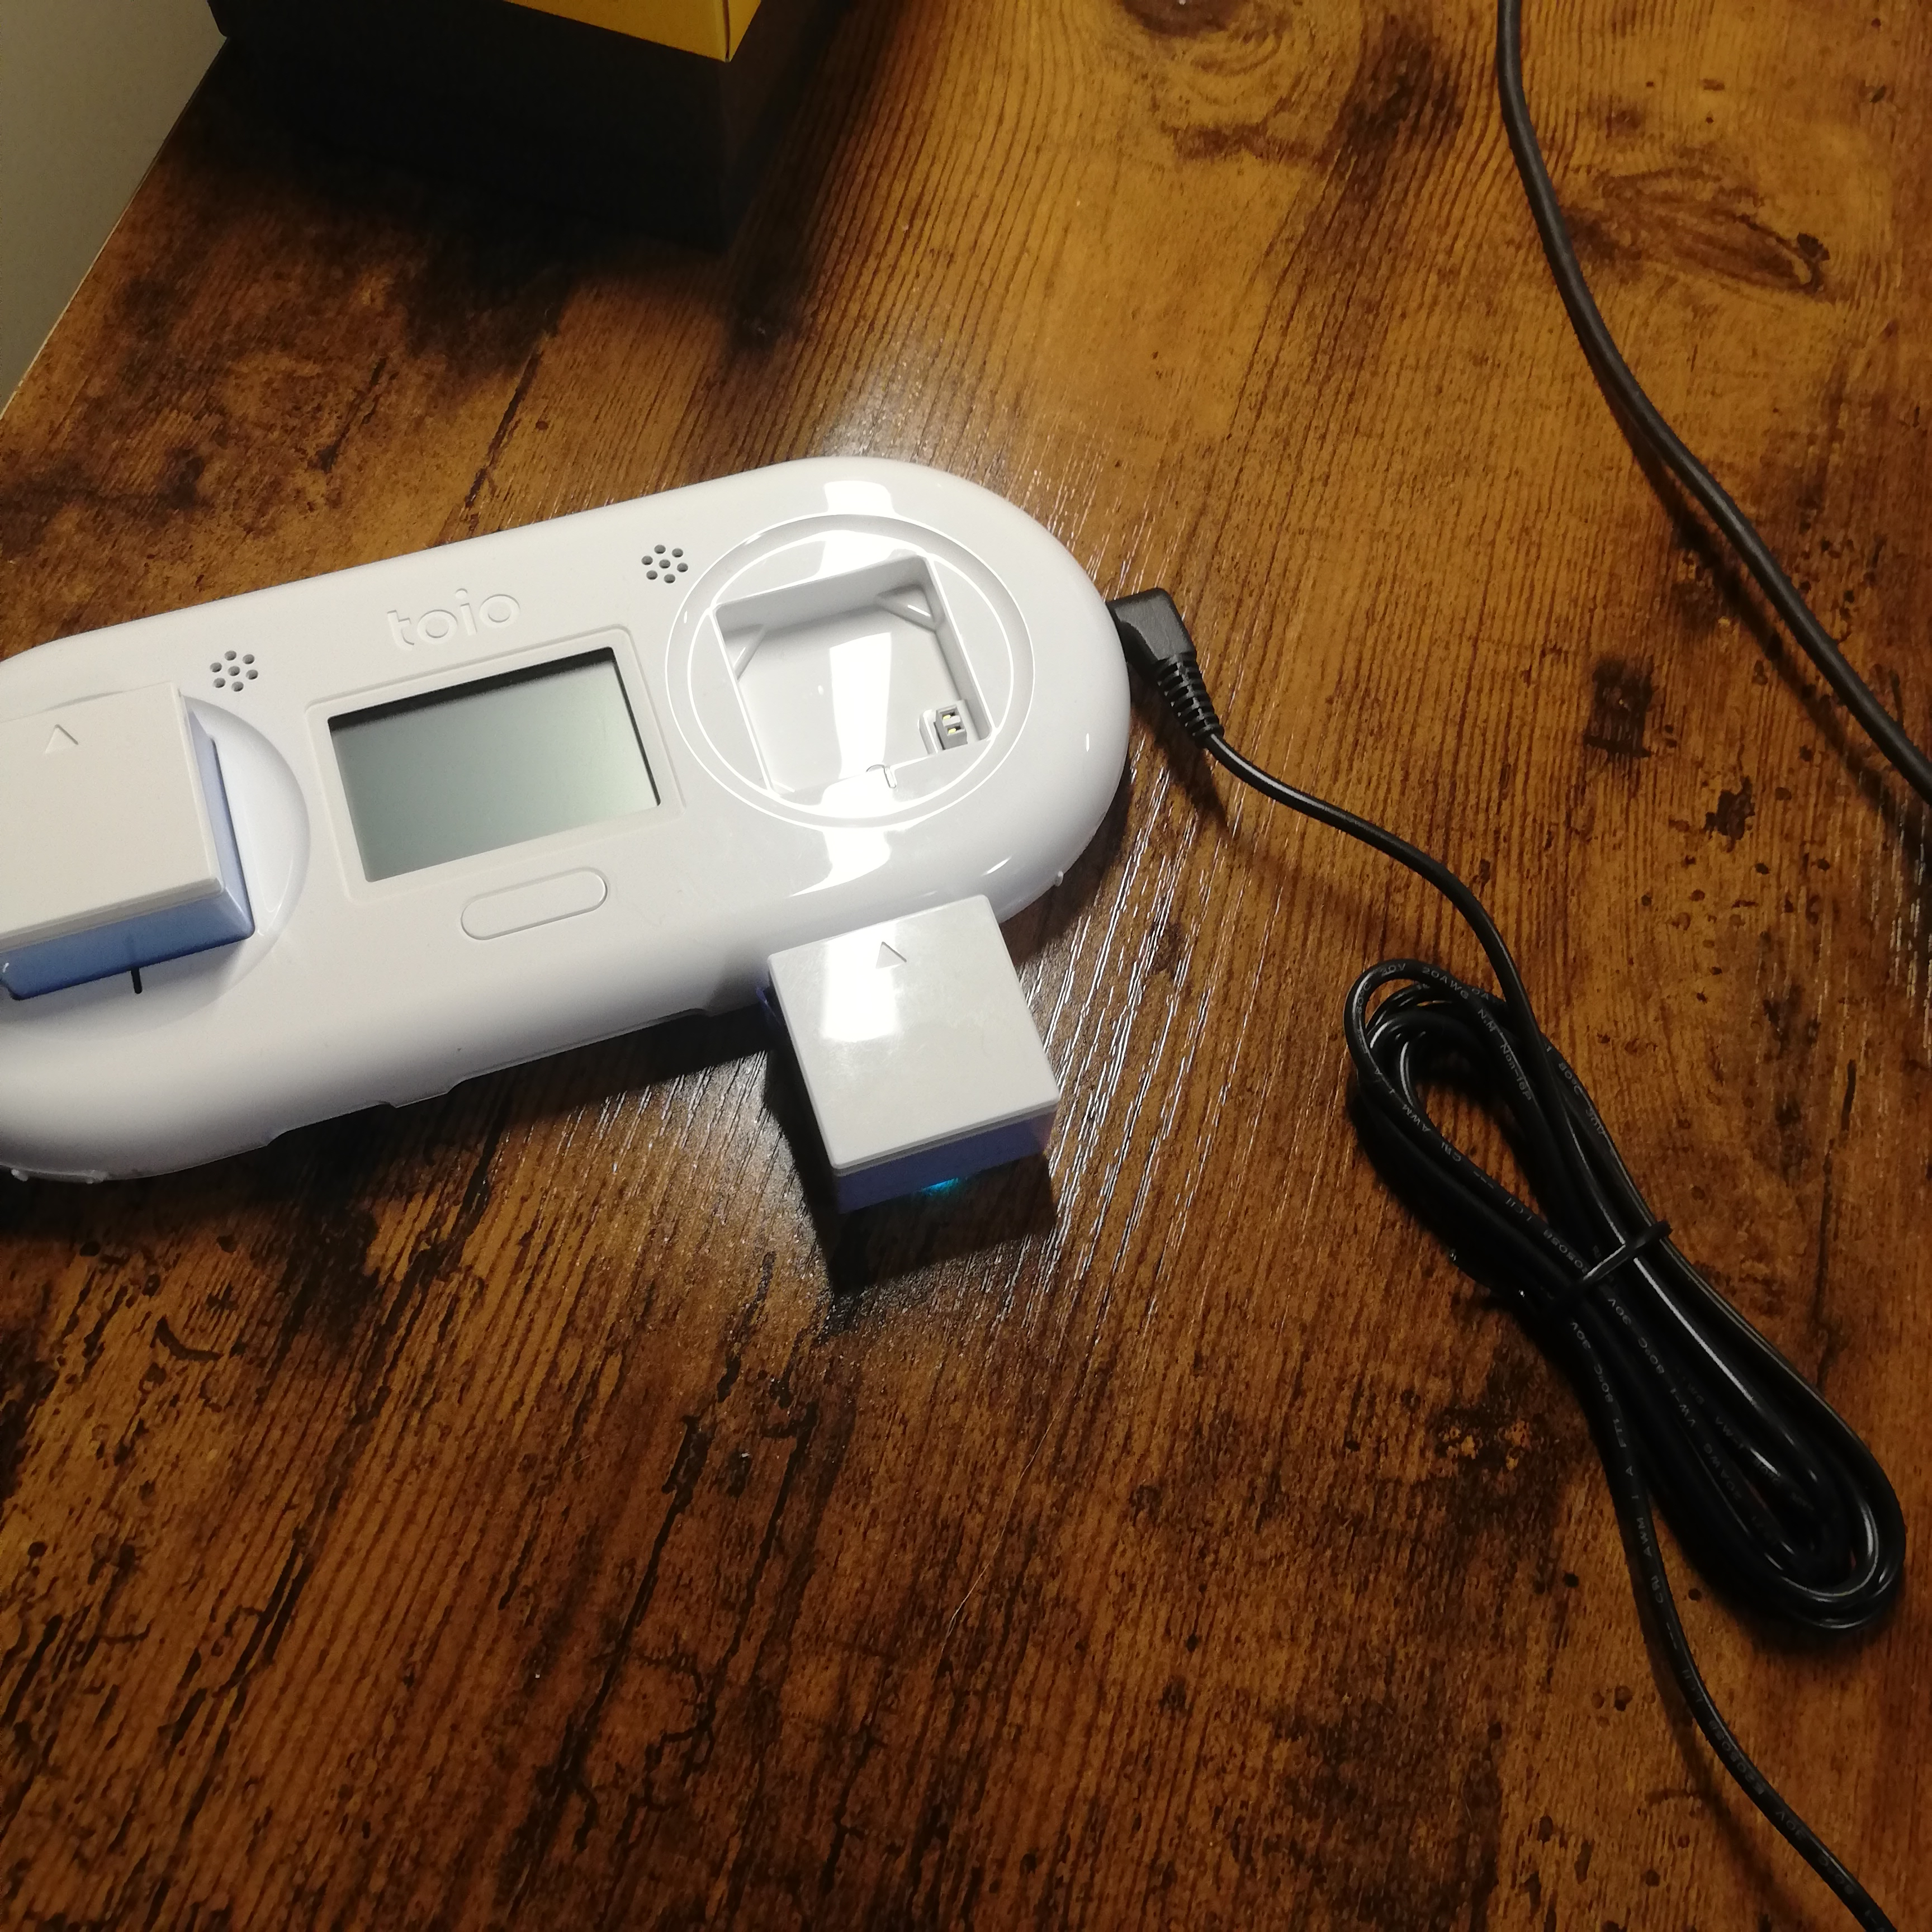
\includegraphics[width=0.9\textwidth]{resources/doc_after.jpg}
    \end{minipage}     &
    \begin{minipage}[c]{0.15\textwidth}
      \centering
      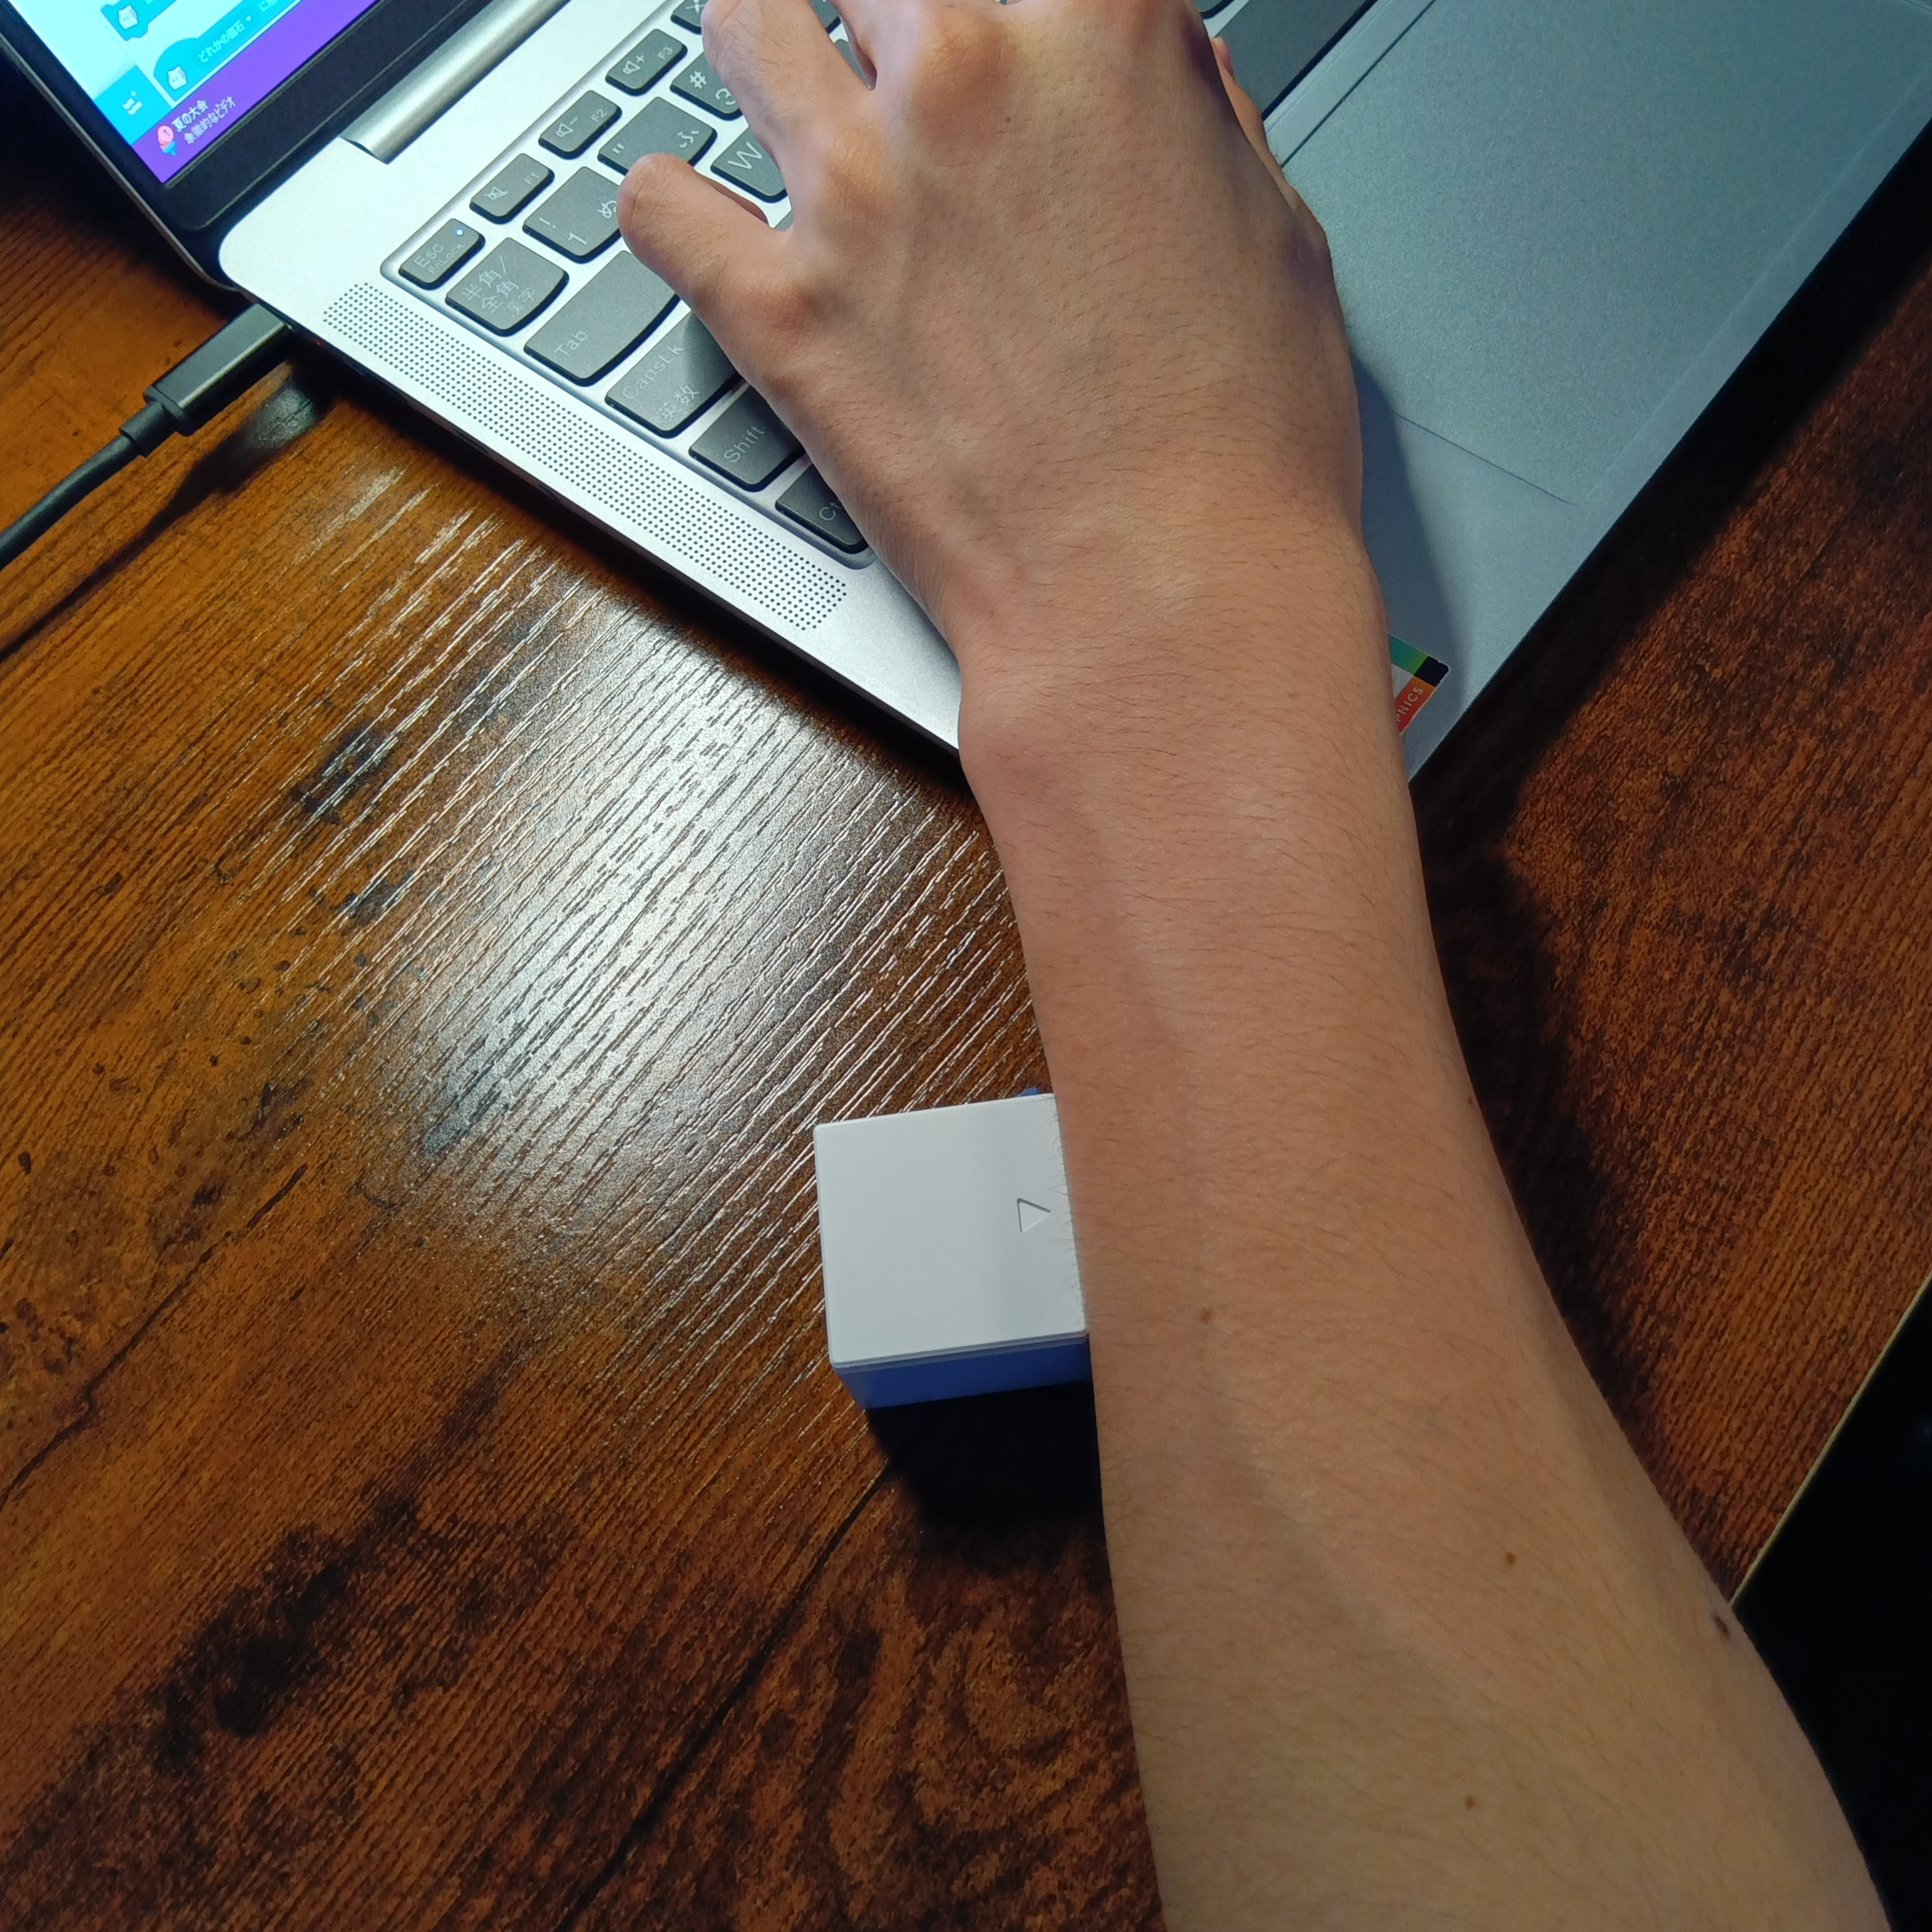
\includegraphics[width=0.9\textwidth]{resources/pet_after.jpg}
    \end{minipage}     &
    \begin{minipage}[c]{0.15\textwidth}
      \centering
      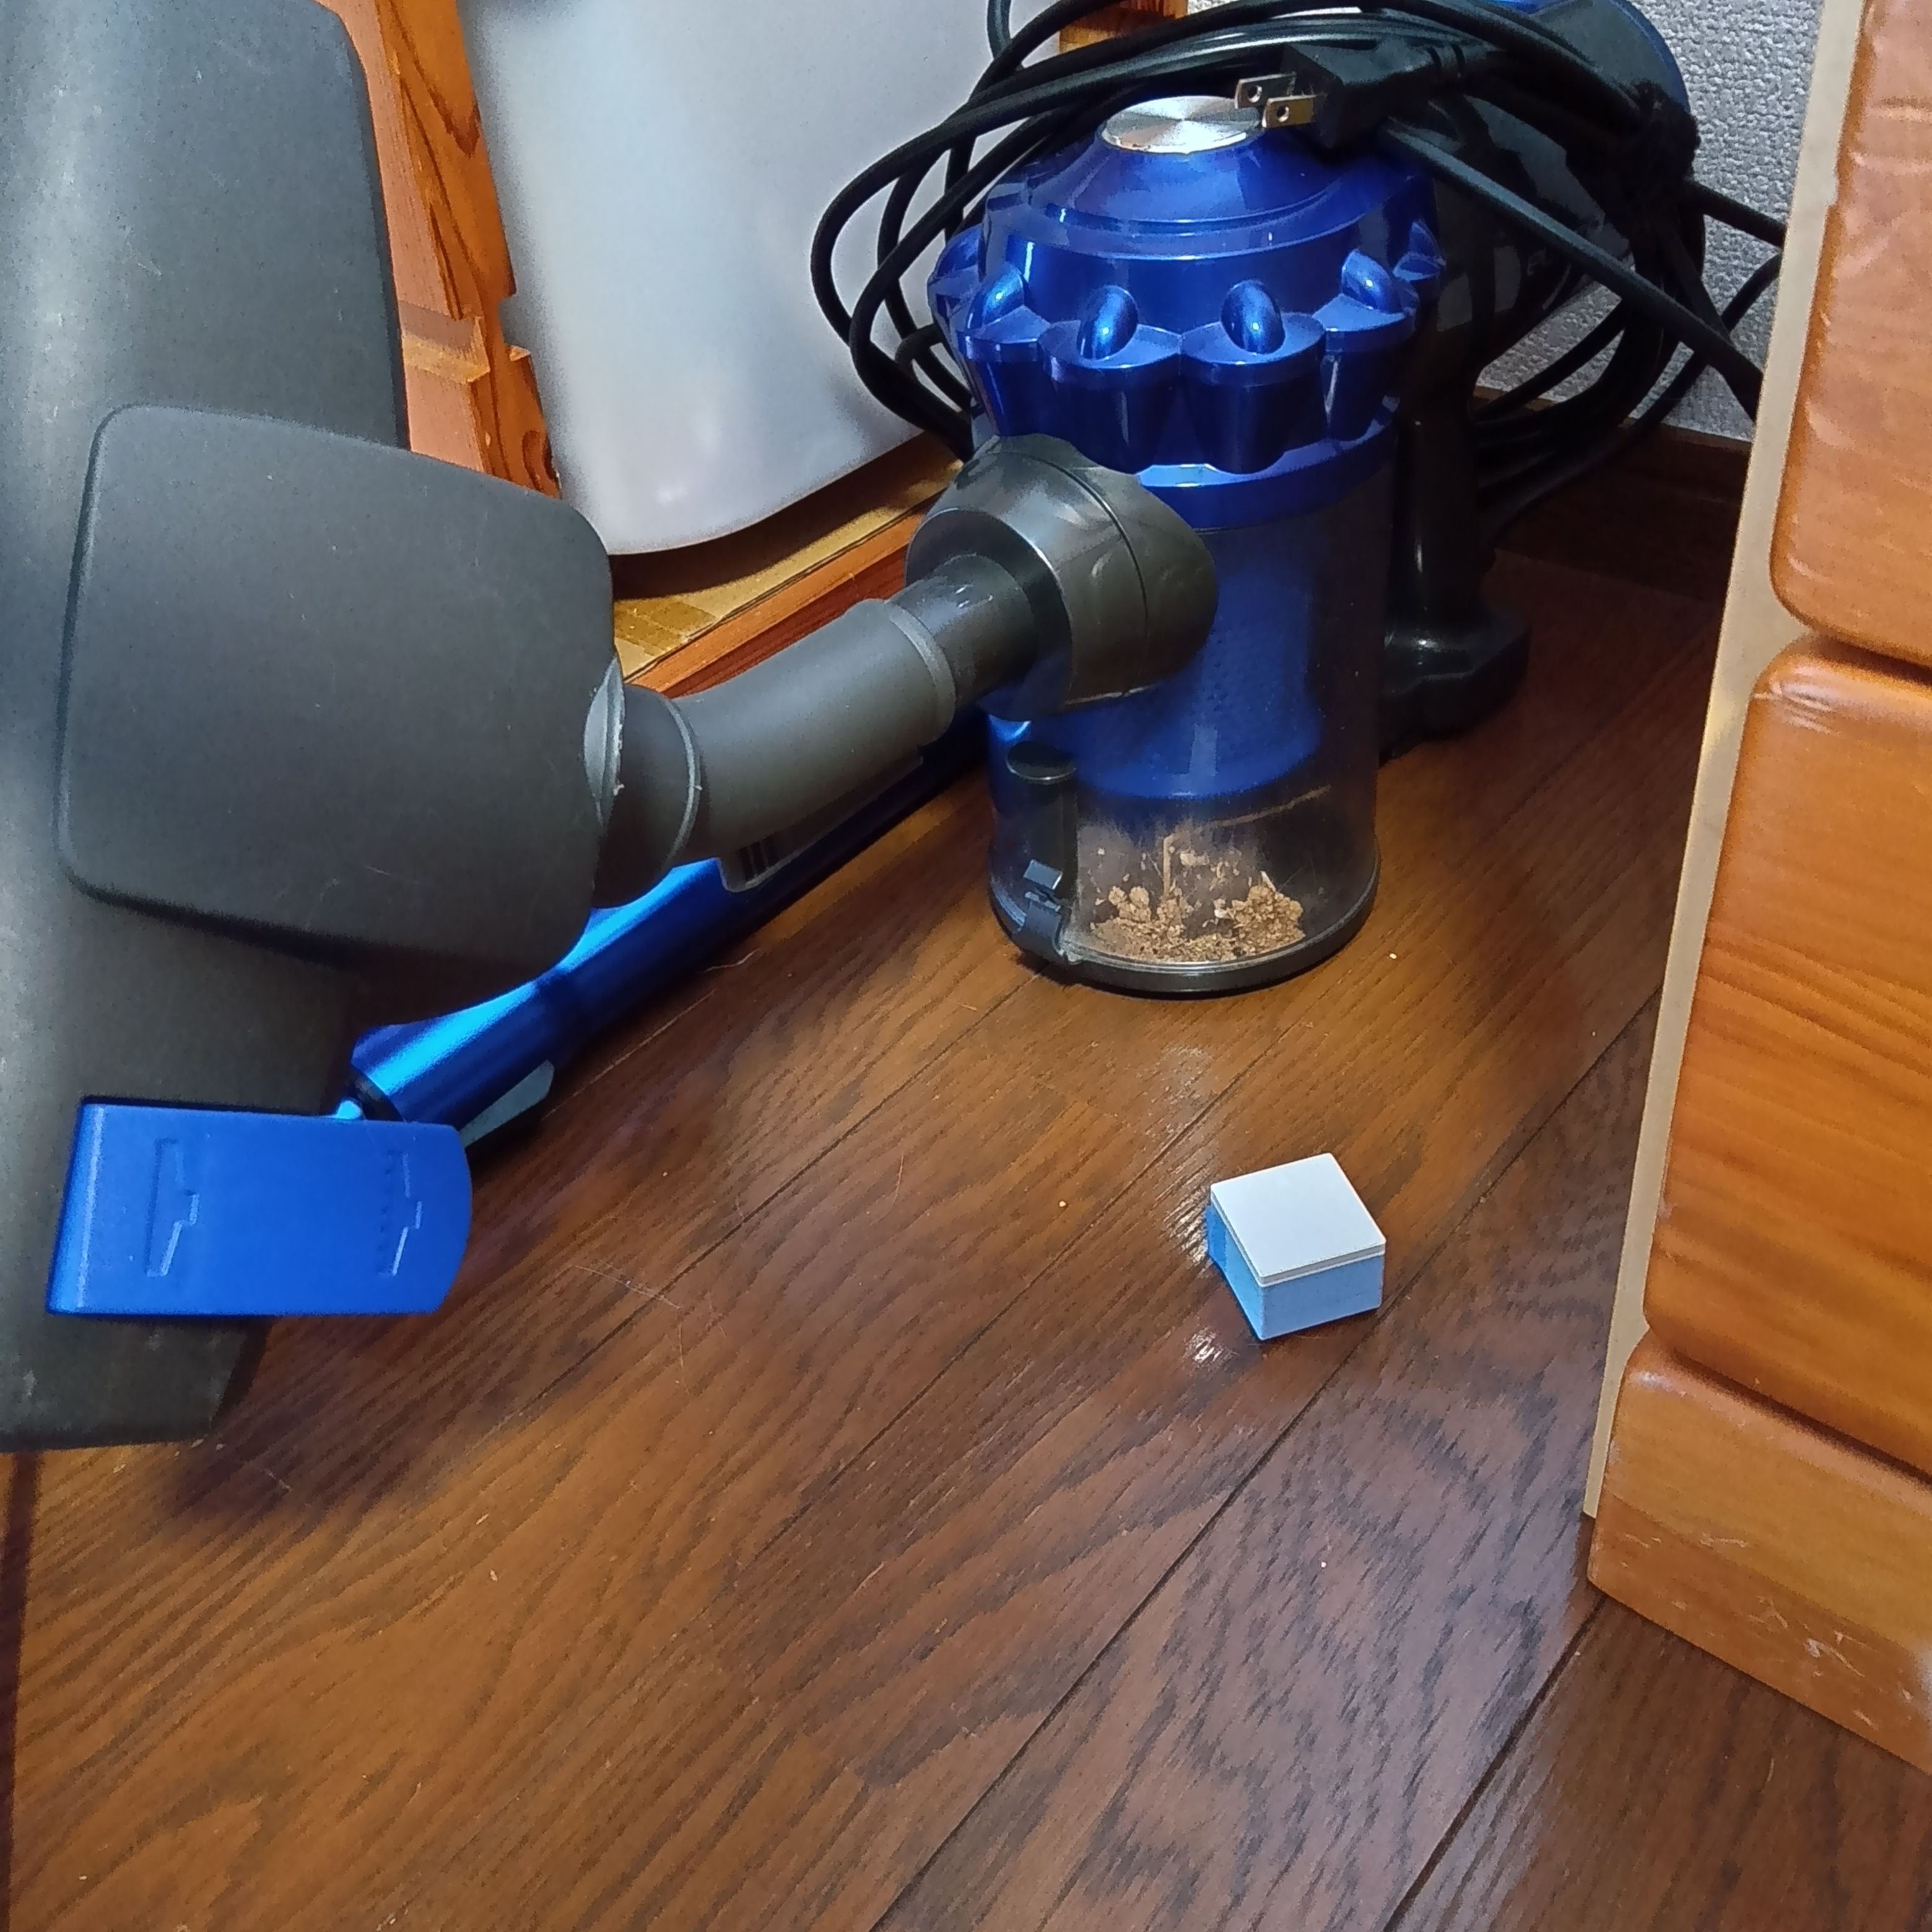
\includegraphics[width=0.9\textwidth]{resources/vacuum_after.jpg}
    \end{minipage}  &
    \begin{minipage}[c]{0.15\textwidth}
      \centering
      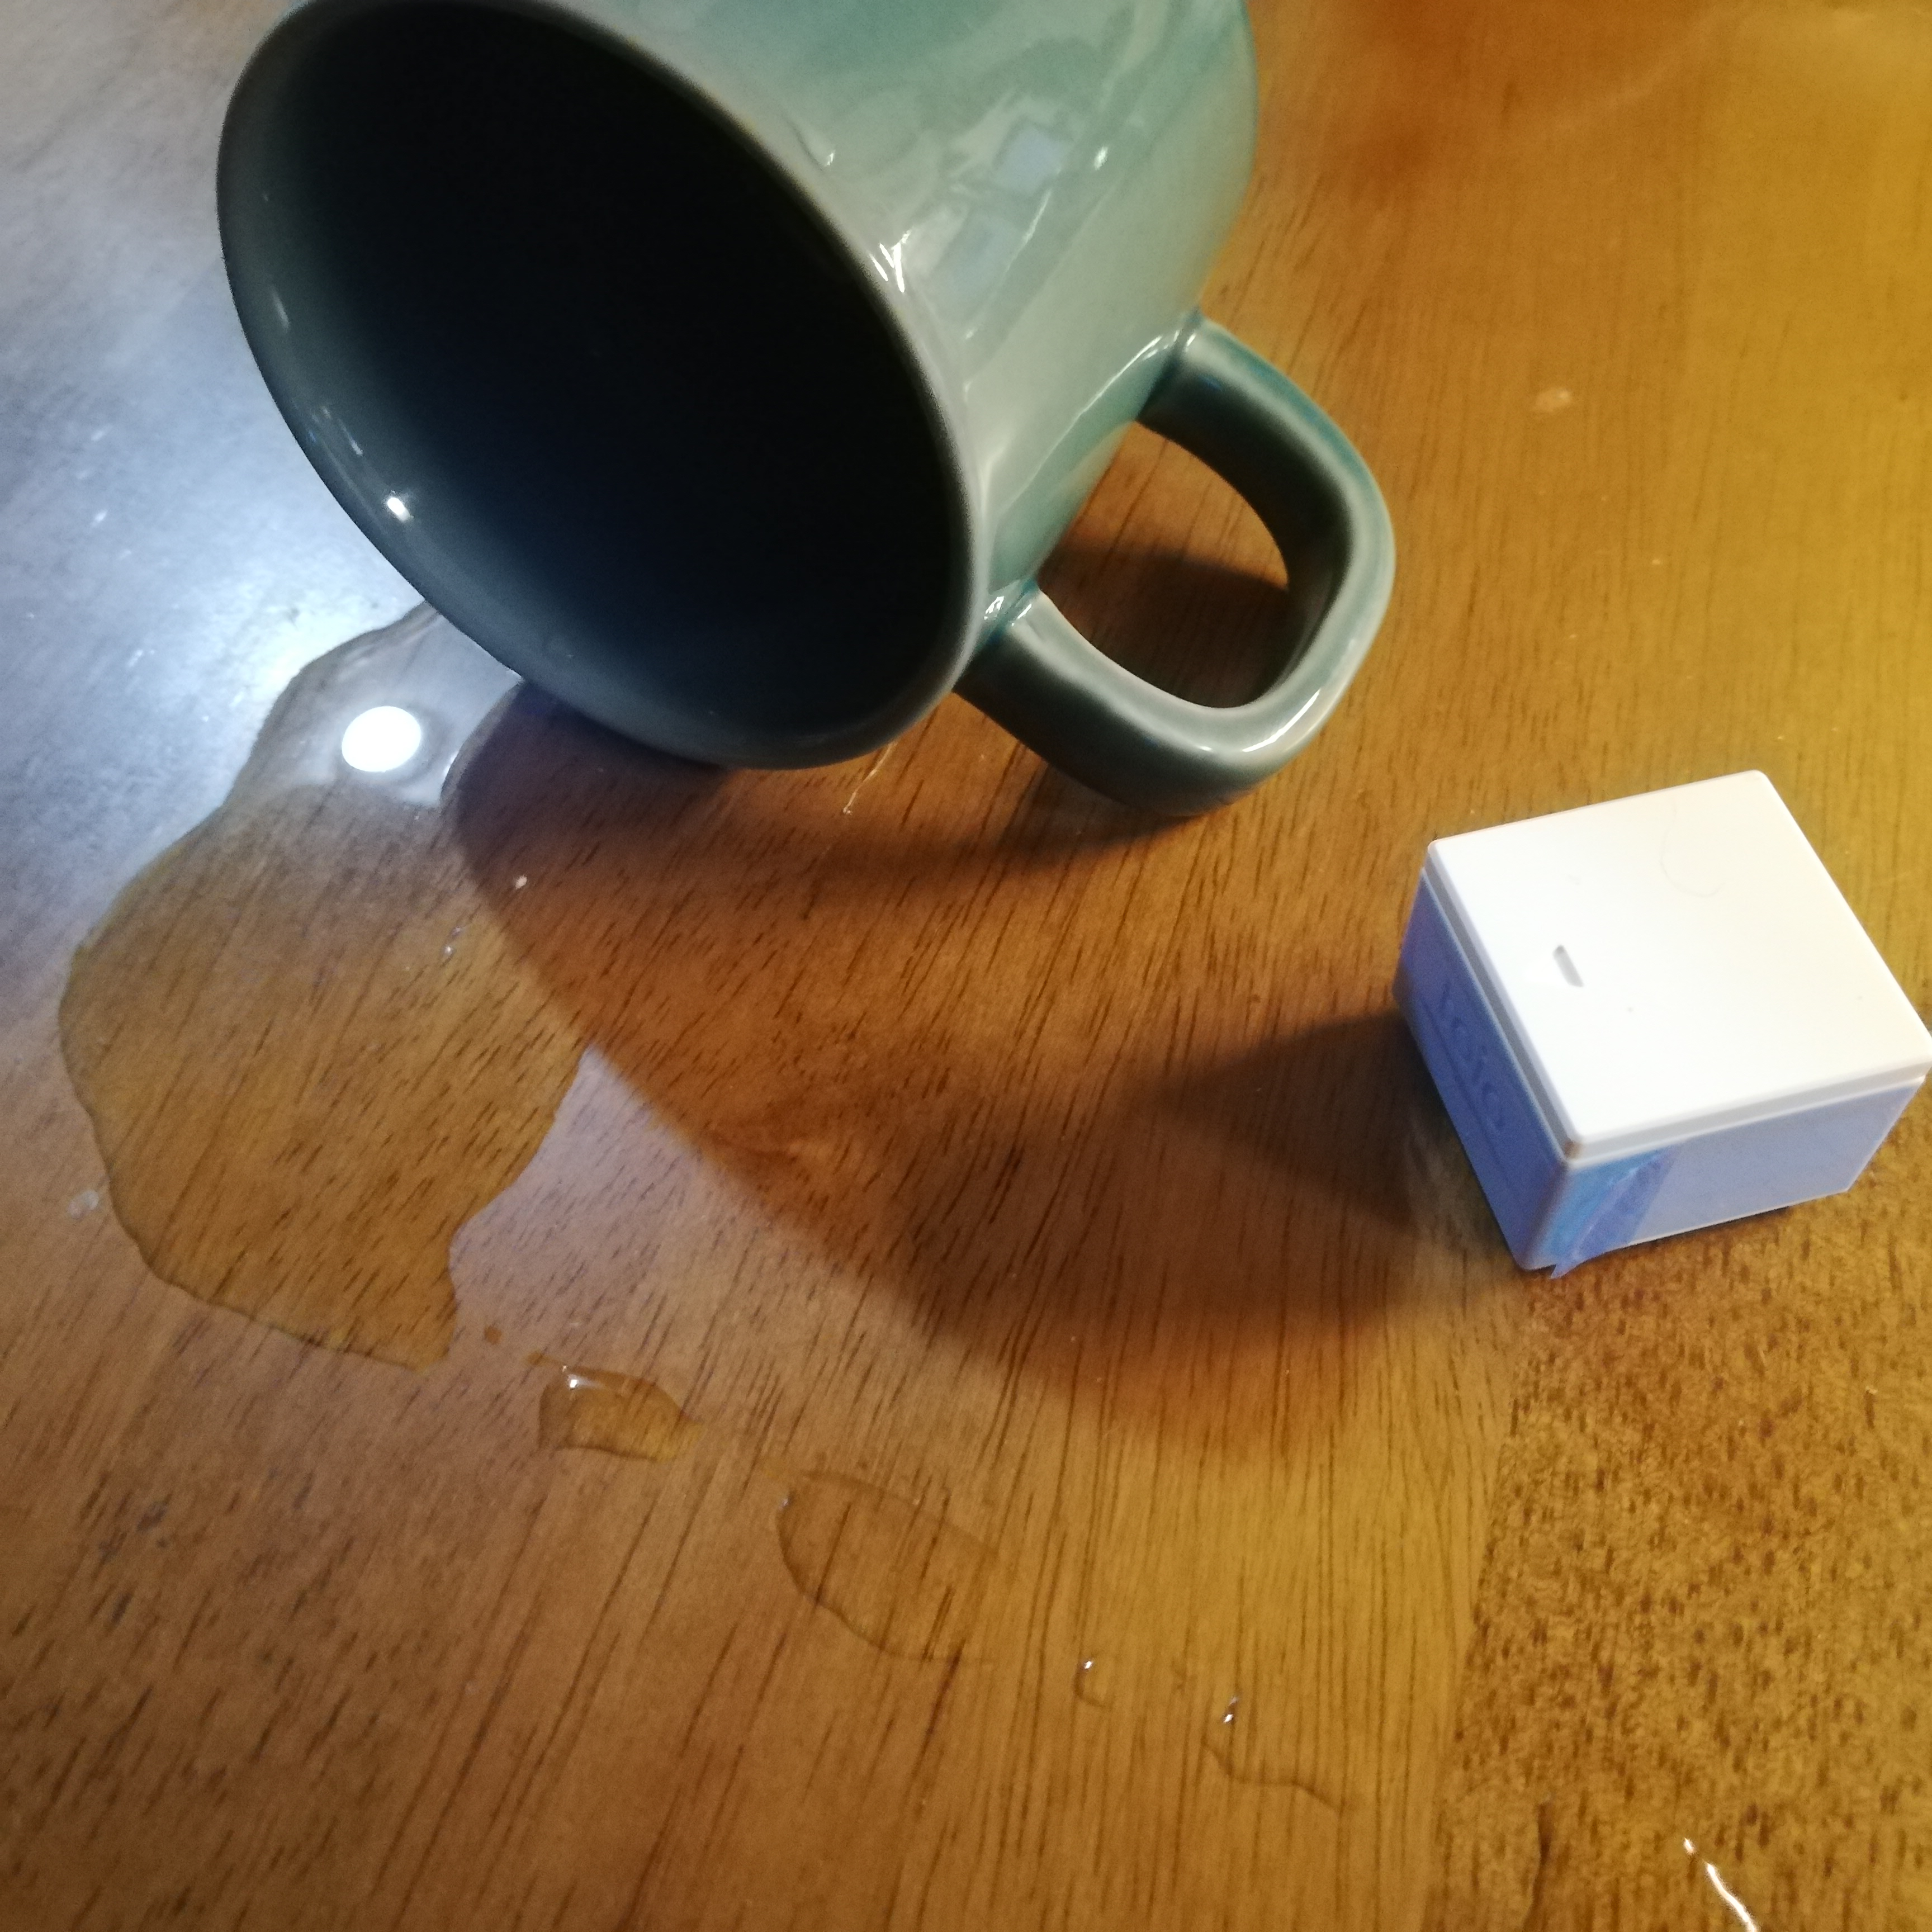
\includegraphics[width=0.9\textwidth]{resources/water.jpg}
    \end{minipage}
    \\ \hline
  \end{tabular}
  \caption{仮置き}
\end{figure*}

本システムの構造を図\ref{fig:system-structure}に示す.

\fboxsep=0pt            %画像と枠線をくっつける.
\fboxrule=1pt            %枠線の太さを1ptにする.
\begin{figure}[h]
  \centering
  \fbox{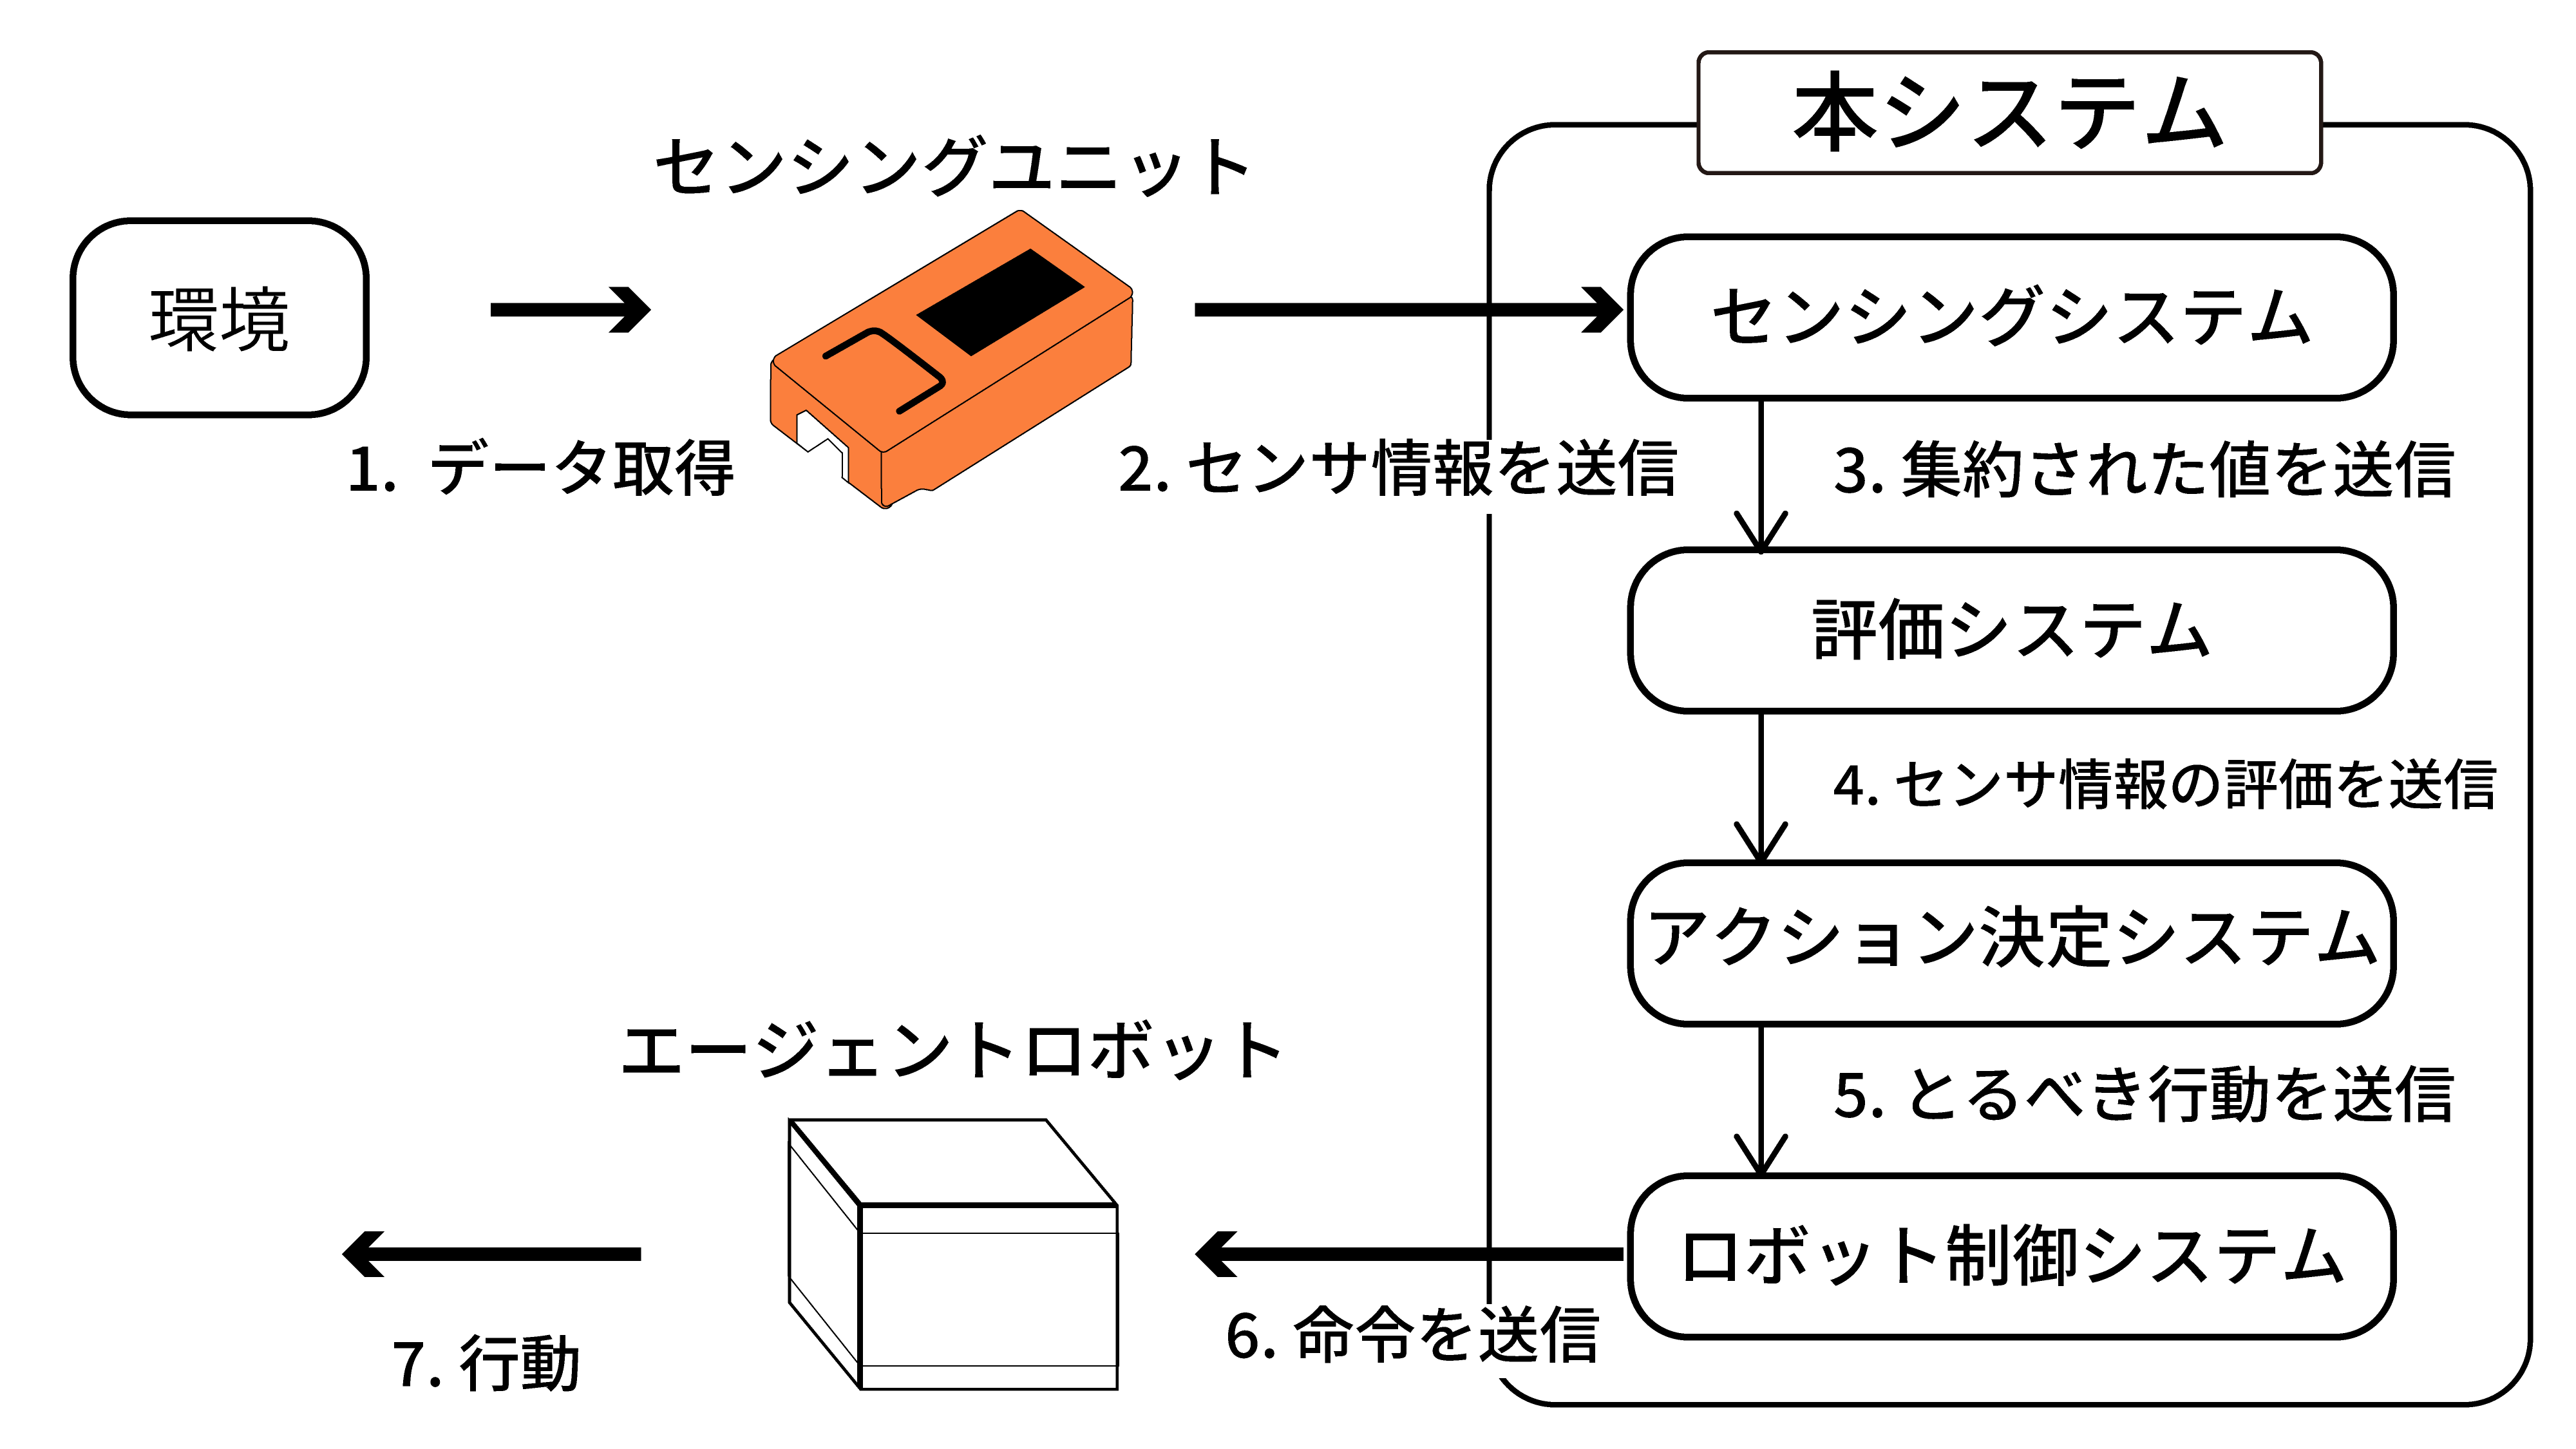
\includegraphics[keepaspectratio, clip,
  width=0.8\columnwidth]{resources/system_structure.png}}
  \caption{本システムの構造図}
  \label{fig:system-structure}
\end{figure}

\subsection{センシングシステム}

センシングシステムは,センサーから送信されたデータを受け取り,以後のシステムにデータを提供する.

\subsection{評価システム}
評価システムでは,センサーシステムから環境データを取得・評価し,評価データを生成する.評価データは,環境データと評価基準値との差をスコアとして所持している.対象データの評価では,例えば人間に適した気温であれば18~24℃などと,あらかじめ対象データの主体にとって最適な範囲を設定する.現在の気温が最適範囲から外れた場合,上回れば正の,下回れば負のスコアをもった評価データを生成する.システム開発者は評価主体とその評価対象ごとに,個別の評価システムを実装する必要がある.

\subsection{アクション生成システム}
アクション生成システムでは,評価システムから取得した評価データをもとに,評価に応じたアクション命令をロボット制御システムへ送る.アクション開発者は,主体および対象の環境データごとにアクションを作成しておく必要がある.サンプルとしてデザインしたアクションには,岡田ら\cite{岡田-2017-弱いロボ}の「弱いロボット」の「よたよた」とした動きを取り入れることで,効果的にユーザーに働きかけることを狙った.

アクションは「コマンド」のキューで構成される.コマンドはロボット動作用のより低レベルな命令と,動作の所要時間を所持しており,一連のコマンドを実行することで,1つの意味あるアクションを表現する.

\subsection{ロボット制御システム}
ロボット制御システムでは,実機toioとシステム上のtoioを識別するためのデータ管理および,アクション生成システムから取得したアクションの実行を行う.

\section{本システムの制約}

提案にあたって,本システムの制約について述べる.

エージェントは,本システムとの通信が可能な範囲に配置する必要がある.今回はBluetooth通信を使用しているため,物理的な仕切りなどによって通信が不安定になりやすい.またエージェントの動作がユーザーから認識できる場所にある必要がある.想定しているエージェントの動作環境は屋内であり,屋外の生活環境での使用は考えられていない.

表現の面では,ロボットが持つモジュールによって可能なアクションが異なる.また本システムが対象とできる他者は,評価基準が明確で,評価データがセンサーによって取得可能なものに限られる.同時に制御できるロボットの数にも制限があるため,大量の他者を同時に表現することは難しい.

\section{今後の展望}
本システムの展望として,アクションデザインでは,ロボットどうしの協調やより効果的な動作のデザイン検討が考えられる.センシング面では,快・不快をより正確に表現するデータの検討や,キャリブレーションの追加等が可能である.また異なるセンサー,ロボットを使用することで,新しいユーザー体験を生み出すことが期待される.

\section{おわりに}
本研究では,環境データを他者の視点から評価し,ロボットの身体的動作を通じて表現するシステムを開発した.M5StickCとtoioを用いたプロトタイプシステムの実装により,他者にとっての快・不快を直感的に理解できるインタフェースを実現した.特に,『弱いロボット』の概念を取り入れることで,ユーザーを自然にシステムフローに組み込むことができた.

今後は,より多様な他者の表現や,ロボット同士の協調動作の実装など,システムの拡張を進めていく.

%  ----- 参考文献 -----
% 参考文献リストの「参考文献」のスタイル
\renewcommand{\refname}{ 参考文献}
\bibliography{ref}
\bibliographystyle{junsrt}
\end{document}
